\documentclass[12pt,a4paper,openright,twoside]{book}
\usepackage[utf8]{inputenc}

\newcommand{\thesislang}{english}
\usepackage{thesis-style}

% version
\newcommand{\versionmajor}{0}
\newcommand{\versionminor}{1}
\newcommand{\versionpatch}{2}
\newcommand{\version}{\versionmajor.\versionminor.\versionpatch}

\begin{document}
	
\frontmatter

% ! TeX root = thesis-main.tex
\title{Title}
\author{Francesca Neri}
\date{\today}

\newgeometry{margin=0.8in}
\begin{titlepage}
	\begin{center}
		% \vspace*{0.2cm}
		
		\large
		\textbf{ALMA MATER STUDIORUM -- UNIVERSITÀ DI BOLOGNA \\ CESENA CAMPUS}
		\\
		\noindent\hrulefill
		\vspace{0.4cm}
		
		%\Large
		Department of Computer Science and Engineering - DISI \\
            \vspace{0.1cm}
        %\Large
		Second Cycle Degree in Digital Transformation Management \\
            \vspace{0.1cm}
            Class: LM-91
		
		\Large
		\vspace{4cm}
		\textbf{
			% The Role of Enterprise Performance Management \\ 
   %          in Modern Businesses: A Case Study of Oracle \\
   %          Cloud EPM Implementation
            Leveraging Oracle Cloud EPM Business Rules \\
            for Efficient Planning: Insights and \\
            Implementation Strategy
		}
		
		\large
		\vspace{2cm}
		Graduation thesis in \\
		\vspace{0.2cm}
		\textsc{BIG DATA AND CLOUD PLATFORMS}
		
		\vspace{5.5cm}
		\begin{minipage}[t]{0.64\textwidth}
			\begin{flushleft}
				Supervisor \\
				\vspace{0.2cm}
				\textbf{Prof. Matteo Francia}
			\end{flushleft}
		\end{minipage}
		\begin{minipage}[t]{0.34\textwidth}
			\begin{flushright}
				Candidate \\
				\vspace{0.2cm}
				\textbf{Francesca Neri}
			\end{flushright}
		\end{minipage}\\
		
		\vfill
		\noindent\hrulefill
		\vspace{0.3cm}
		\large
		
		I Graduation Session
		\\
		Academic Year: 2022-2023
	\end{center}
\end{titlepage}
\restoregeometry


\begin{acknowledgements}

%I would like to express my gratitude to PwC Italy for this opportunity, to the entire EPM team for welcoming me and making me feel like a part of the team, and my supervisor for his guidance and support throughout the internship. \\

\end{acknowledgements}

\begin{abstract}	

This thesis explores the potential of leveraging Enterprise Performance Management (EPM) to enhance planning efficiency in modern businesses. 
%
The project was carried out using Oracle Cloud EPM, a cloud-based platform developed by Oracle Corporation, which offers an integrated suite of financial and operational planning and analysis tools.
%
The study provides valuable insights and details on the implementation strategy specifically focused on harnessing the capabilities of Oracle Cloud EPM and its business rules for optimal planning outcomes.

The thesis starts by providing the background and significance of the project, highlighting the need for efficient planning in organizations. The scope and objectives of the study are defined, along with the project requirements. An overview of the methodology employed throughout the research is also provided.
%
The main focus of the thesis regards the exploration of how financial and operational processes are integrated in a single EPM solution, whilst using data coming from different sources.
%
It dives into the implementation of an EPM solution, with a specific focus on the role of business rules in driving efficient planning within Oracle Cloud EPM. 
%
The project involved working with a real-world organization to identify the planning needs and goals.

The goal of this project is to provide a detailed exploration of the role of EPM solutions in modern business, with a focus on valuable insights and implementation strategies in the optimization of performance management.
%
The project provides a practical example of how businesses can leverage EPM solutions to improve their financial and operational planning and analysis capabilities.

\end{abstract}

\begin{dedication}
Optional. Max a few lines.
\end{dedication}

% \begin{acknowledgements}
% Optional. Max 1 page.
% \end{acknowledgements}

%----------------------------------------------------------------------------------------
\tableofcontents   
%\listoffigures     % (optional) comment if empty
%\lstlistoflistings % (optional) comment if empty
%----------------------------------------------------------------------------------------

\mainmatter

%----------------------------------------------------------------------------------------
\chapter{\introductionname}
\label{chap:introduction}
%----------------------------------------------------------------------------------------

This thesis is linked to my curricular internship for the final examination carried out at PricewaterhouseCoopers (PwC) from January to March 2023.
%
During the internship experience at PwC Italy, I worked in the advisory-transformation Line of Service, cooperating with the Enterprise Performance Management - Financial Service (EPM-FS) team.
%
The EPM-FS team works for the main players in the financial sector and deal with business transformation projects which are aimed at re-engineering and optimizing the company's internal processes.
%
Along the internship period, I worked directly with the EPM team in a project concerning the Oracle Cloud EPM platform.
%
This project is addressed to an Italian Holding Group which has more than 7,000 points of sale around the world. 
%
Due to corporate policy, the name, data and information of the Holding Group to which the project is addressed, cannot be disclosed. 
%
It is important to note that respecting the privacy and confidentiality of companies' data is critical in maintaining their trust and credibility.
%
Therefore, throughout this thesis, I will be referring to the company only in general terms and avoiding the use of any identifying information or data.

In today's highly competitive business environment, effective performance management is essential for organizations to achieve their strategic goals and stay ahead of the competition.
%
With the advent of digital transformation, companies are now offered with huge opportunities from which they can benefit.
%
It is an inevitable change that organizations must embrace to stay competitive and meet customer demands in the digital era.
%
One of the way to go in order to thrive among rivals in turbulent markets is to excel at various performance dimensions. 
%
One of the prerequisites for this is to be able to effectively manage and measure corporate performance using various performance management and measurement systems. 
%
These systems help companies to continuously react and adapt to external changes.

Enterprise and corporate performance and management methods can be viewed as the seamless integration of managerial systems. 
%
Each method should be embedded with business analytic operations to provide valuable data and insights that can help businesses make informed decisions by identifying trends, anticipating issues, and making adjustments to their strategy as needed.
%
Enterprise Performance Management (EPM) is an integral part of the success of modern enterprises as it helps organizations to gain visibility into their performance and to identify areas of improvement.
%
It is a management approach that integrates multiple business processes and systems to enable organizations to plan, measure, analyze, and optimize their performance.

Enterprise Performance Management enables businesses to improve strategic decision-making, maximize their productivity and achieve the desired business results while ensuring that expenses are minimized and that the best use of resources is made.
%
It assists businesses to effectively forecast and plan for their future financial performance, helping them to ensure compliance and reduce risk. 
%
The advantages of EPM are numerous and make it a valuable tool for organizations of all sizes.

The aim of this thesis is to investigate the role of EPM in modern businesses and the benefits and challenges of implementing EPM solutions. 
%
Specifically, this thesis will focus on a practical case of Oracle Cloud implementation for a business to illustrate how EPM solutions can improve organizational performance. 

Oracle Cloud is a leading cloud-based EPM solution that provides organizations with a comprehensive suite of financial and operational performance management applications.
%
Oracle Cloud EPM provides a flexible and scalable solution that can meet the needs of organizations of all sizes.
%
It offers various tools and solutions that allow companies to plan, budget, forecast, and report on their financial and operational performance.
%
The implementation of an Oracle Cloud EPM solution involves a series of steps throughout which organizations must work closely with their implementation partner to ensure that the solution is tailored to their specific needs and requirements.
%
Using a cloud platform to implement an EPM solution can provide numerous benefits for the organization. 
%
One of the primary advantages regards the ability to access critical data and applications from anywhere and at anytime.
%
Additionally, cloud platforms can help reduce costs associated with maintaining on-premises infrastructure and provide scalability and flexibility to meet changing business needs. 
%
Cloud-based EPM solutions also enable organizations to leverage the latest technologies and innovations without having to worry about managing and upgrading hardware and software. 
%
Cloud providers typically offer high levels of security and compliance, which can help organizations protect sensitive data and maintain regulatory compliance. 

\newpage

\paragraph{Thesis Structure.}
%

Accordingly, the reminder of this thesis is structures as follows:
%
\Cref{chap:introduction} provides an overview of the background and significance of the project.
%
The chapter outlines the scope and objectives of the project, highlighting the specific areas that will be addressed. 
%
Additionally, the project requirements are defined, and an overview of the methodology used in the study is presented. 
%
This chapter serves as an introduction to the thesis, setting the stage for the subsequent chapters to delve deeper into the topic of efficient planning using Oracle Cloud EPM.
%
\Cref{chap:epm} explores the concept of Enterprise Performance Management. 
%
It defines EPM and provides an understanding of its key concepts and components. 
%
The chapter discusses the benefits that organizations can achieve by implementing EPM and highlights the challenges that may arise during the implementation process. 
%
This chapter aims to establish a foundation of knowledge regarding EPM, laying the groundwork for the subsequent chapters.
%
\Cref{chap:implementation} focuses on the implementation of Oracle Cloud EPM. 
%
It begins with discussing the process of selecting an EPM solution and outlines the key considerations involved in the decision-making process. 
%
The chapter then explores the elements of the implementation process, providing insights into the steps required to successfully deploy Oracle Cloud EPM. 
%
Additionally, it discusses the importance of building a comprehensive EPM solution, emphasizing the integration of various modules and functionalities. 
%
The chapter also addresses data transformation and calculations, introducing Business Rules and highlighting their significance in optimizing the use of Oracle Cloud EPM.
%
\Cref{chap:cmyactivity} delves into the concept of Business Rules and how they can enhance efficient planning within Oracle Cloud EPM. 
%
It examines two practical implementations: cost allocation and intercompany management. 
%
The chapter explores the implementation of business rules in these domains, providing insights into the best practices and strategies for achieving efficient planning outcomes. 
%
By exploring these specific use cases, the chapter aims to provide practical guidance and actionable recommendations for leveraging Oracle Cloud EPM business rules.
%
Finally, \Cref{chap:conclusions} offers a summary of the entire project. 
%
It recaps the main points discussed in each chapter, highlighting the key findings and insights. 
%
The chapter also includes a discussion section where the implications of the research findings are analyzed and interpreted. 
%
Finally, the chapter presents concluding thoughts, offering a reflection on the overall study and its contribution to the field of efficient planning using Oracle Cloud EPM.

\section{Background and significance of the study}

Enterprise Performance Management is a management approach that involves using data and analytics to monitor, measure, and improve an organization's performance. 
%
It integrates various management processes, including financial planning, budgeting, forecasting, risk management, and performance measurement, to help organizations to align their goals with their strategies and improve their overall performance.
%
To access and analyze data more quickly and accurately, organizations typically use software applications that automate and streamline this process.
%
These applications often include dashboards, pre-built report templates and other tools that provide real-time insights into organizational performance.
%
By using data-driven insights and decision-making, EPM enables organizations to more effectively manage risks, allocate resources, and make strategic decisions that improve their overall performance and competitiveness in the marketplace.

Enterprise Performance Management operates within a complex and dynamic business environment, characterized by a number of key trends and challenges. 
%
One of the most significant trends in recent years has been the growing adoption of cloud technology for enterprise applications, including EPM. 
%
Cloud-based EPM solutions offer many advantages over traditional on-premises systems, including greater scalability, flexibility, and accessibility, as well as lower costs and reduced IT complexity. 
%
As a result, more and more organizations are turning to cloud-based EPM solutions to improve their performance management processes.
%
Another key trend in modern business is the growing importance of data-driven decision making. 
%
With the increasing availability of data and advanced analytical tools, organizations are able to gain deeper insights into their operations and performance, and make more informed decisions. 
%
EPM plays a critical role in this trend by providing real-time insights into organizational performance and enabling managers to make data-driven decisions that align with their strategic goals. 
%
This helps organizations to be more proactive in identifying and responding to performance issues, and to optimize their operations and resources to achieve their desired outcomes.

In addition to these trends, EPM also operates within a business environment that is constantly evolving and adapting to changing market conditions. 
%
The need for businesses to be agile and responsive to these changes is an ongoing challenge, and EPM can help address this by providing a flexible and adaptable framework for performance management. 
%
By monitoring key performance indicators and providing real-time insights into performance, EPM enables businesses to quickly identify and respond to changes in market conditions, and to make strategic decisions that keep them ahead of the competition.
%
The context in which EPM operates is characterized by a rapidly evolving business environment, where technology, data, and agility are critical to success. 
%
It plays a critical role in helping organizations to adapt to these trends and challenges, by providing a data-driven and agile approach to performance management that enables them to optimize their operations, resources, and strategic decision making.

\section{Scope and objectives of the project}

The EPM implementation project has been implemented for a Holding Group, which is a global leader in high-end design with pro-forma revenues of \$ 960 million in 2022.
%
The Holding Group is characterised by an unparalleled portfolio of iconic Brands and a multi-channel distribution approach across the globe.
%
Its mission is to provide long-lasting value for clients through an innovative manufacturing process carried out by the Brands which compose the Holding Group.
%
It is composed of ten brands which own a total amount of ten factory locations in Italy, Spain, Denmark and US.
%
The Holding Group has a presence in more than 130 countries with more than 7,000 points of sale worldwide. 
%
They created an exclusive network of highly professional dealers and mono-brand stores, consolidating its international presence with the opening of wholly owned flag-ship stores in leading capital cities around the world.

Their goal is to foster an ecosystem which enables their companies to grow into a strong worldwide presence with both reach and scale by curating a powerful and iconic culture across the Brands.
%
This ecosystem has been geared towards the success of each individual Brand, so that the Holding Group invests its resources at Brand level, boosting the creative process and the customer experience.
%
By bringing together multiple Brands and helping them achieving their best, the Holding Group is a global leader in an otherwise traditionally highly fragmented market of high-end design. 
%
With a strong cultural heritage, characterised by multi-channel distribution and diversified product categories, the Holding Group has created a unique design hub, offering a platform with which carefully selected Brands can be accelerated to grow at scale through a well-defined strategic approach.
%
Their strategic pillars are:

\begin{enumerate}
    \item Brand desirability, making Brands more attractive, better known and sought after.
    \item Direct to consumers, enhance and personalize the customers’ experience, getting closer to end customers and the design community.
    \item International expansion, expand the geographical reach, boosting their presence in markets with high growth potential and building a strong position into mature ones.
    \item Contract business, strengthen the leadership in high-end Contract business, providing considerable added value to the overall quality of a project in the eyes of architects, designers, and developers.
\end{enumerate}

\begin{figure}[h]
	\centering
	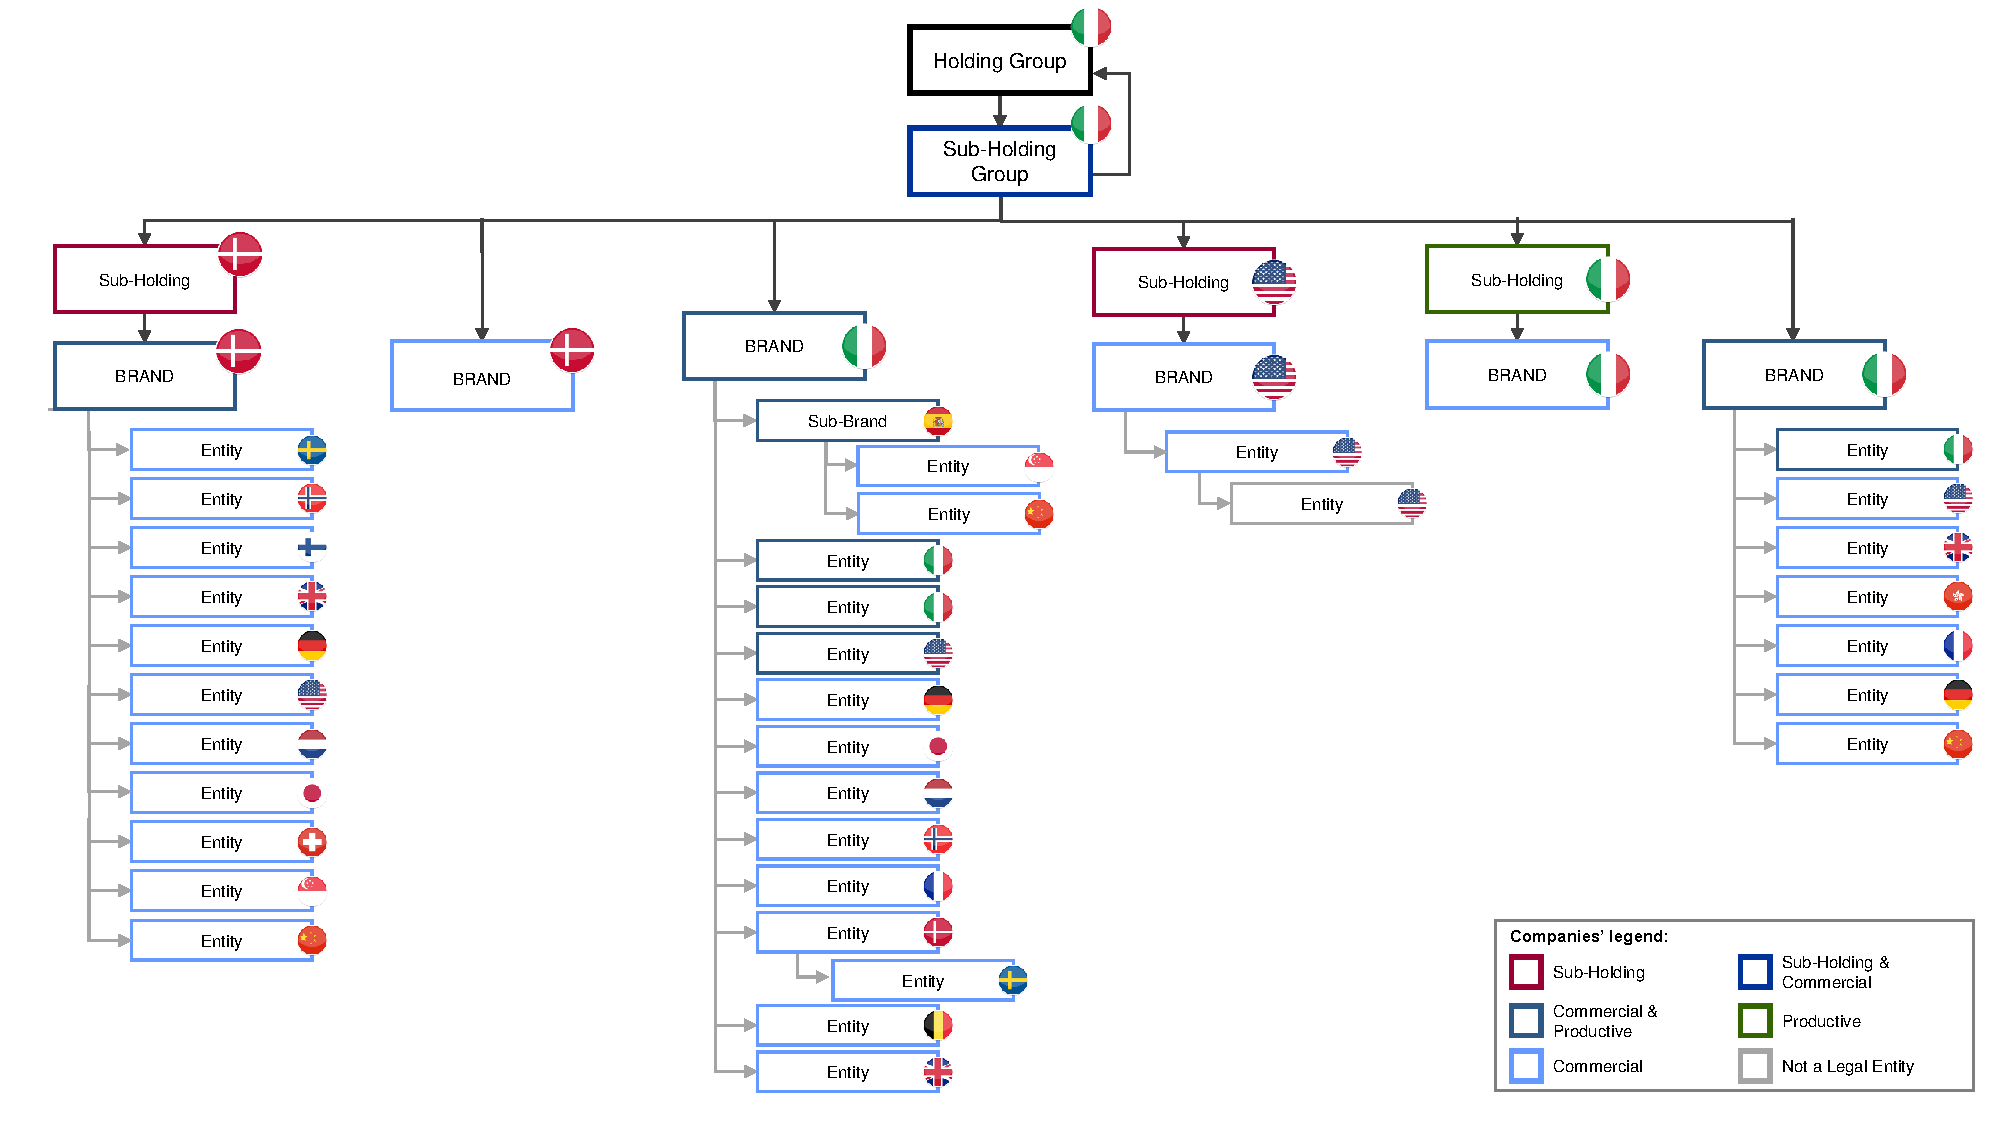
\includegraphics[width=\linewidth]{figures/structure.pdf}
	\caption{Structure of the Holding Group}
	\label{fig:structure}
\end{figure}

The Management Control Department\footnote{Management Control in a business refers to the processes and activities undertaken by a dedicated department to plan, monitor, and control organizational activities. The aim of management control is to align the actions of individuals and departments with the company's strategic goals and objectives, enabling effective decision-making, performance evaluation, and the optimization of resources.} of the Holding Group is responsible for assessing the financial situation and evaluating the overall performance of the Entities.
%
Their tasks and activities range from monitoring financial performance, tracking key performance indicators (KPIs), and identifying areas for improvement.
%
Prior to the implementation of the Enterprise Performance Management solution, the Management Control Department faced significant challenges in accessing and consolidating financial data from across the Entities.
%
This made it difficult to accurately evaluate performance and to make informed decisions.
%
With the EPM solution, the Management Control Department plans to improve data accuracy, streamline reporting processes, and gain real-time visibility into financial data across all Entities. 
%
The final goal is to drive better decision-making and improve overall financial performance for the Holding Group and, ultimately, make informed decisions that lead to growth and increased profitability. 
%
Additionally, the increased efficiency and productivity that comes with a cloud EPM solution can help to reduce costs and improve compliance and risk management.

The goal of the project is to implement a planning environment in Oracle Cloud EPM in which the data belonging to the different Brands and Entities of the Holding Group are all integrated in a single view.
%
Therefore, the implementation project involves the deployment of a software solution that will enable the company to effectively manage its financial data, analyze it, and make informed business decisions.
%
In particular, the planning environment is used an maintained by the Holding Group Management Control Department so, along the implementation process, we interacted directly with the people working in that area.

The Holding Group was born in 2018 as the result of the aggregation of different Entities which belong to the same industry sector, as illustrated in figure \ref{fig:structure}
%
The Entities which compose the Holding Group have a different story, a different culture, different business models and, as a consequence, different control models.
%
Since its creation, the Holding Group has planned several initiatives to facilitate the integration between the different realities.
%
The lack of organizational structure due to the different control models was considered as a key issue in sustaining the new planning and reporting needs of the Holding Group.
%
To solve this issue, the Holding Group started an activity of homogenization of Enterprise Performance Management of the Entities, by:

\begin{enumerate}
    \item Defining a consolidated financial reporting;
    \item Defining a performance reporting system based on KPI’s;
    \item Defining a treasury reporting and rolling cash flow forecast process\footnote{Treasury reporting refers to the process of generating and presenting financial information related to the organization's cash and liquidity management activities, while rolling cash flow forecast process involves regularly projecting and updating the organization's anticipated cash inflows and outflows over a specified period.}.
\end{enumerate}

The objective of the Holding Group is that of gaining visibility and control over the group's performance with an homogeneous and consolidated reporting activity.
%
They plan to achieve a deep visibility on the single performances, in order to extract insights and KPIs from entities independently.
%
At the same time, the Entities which are part of the Holding Group necessitate a clear consolidation process and homogeneous reporting.
%
For them, it is important to achieve high reliability on data and reporting, thus enhancing data quality, as well as enlarging the Enterprise Performance Management model at Entity level to extract analytics locally.

The project implementation goes around three main macro-areas, which are financial reporting, management reporting and performance analysis.
%
Financial reporting is mandatory for businesses and is mainly used for external purposes.
%
Financial reports include the Profit and Loss Statement, Income Statement, Balance Sheet, Accounts Payable, Accounts Receivable and the Statement of Cash Flows.
%
These reports are important for stakeholders like banks, investors and regulators, to ensure that the company is following accounting standards correctly.
%
Financial reporting reflects the financial position of a business at the time of reporting, however, they cannot be used to predict future performance or provide insights.

Management reporting is optional and is for internal business purposes. 
%
Management reports aim to dive deeper into the company financials and provide insights that enable more informed business decisions. 
%
Management reporting focuses on individual areas of the business, allowing companies to identify areas that are strong and any area of potential improvement. 
%
For example, they might want to see how well the sales department is performing one month before making the decision to expand. Management reporting for performance management enables leaders to rely on their numbers.

Performance analysis, on the other hand, is the process of evaluating the performance of a business, product, service or process against established benchmarks and objectives. 
%
It involves collecting and analyzing data to identify patterns, trends, and opportunities for improvement.
%
Performance analysis is particularly important for businesses because it helps them to identify areas of strength and weakness, improve efficiency and productivity, reduce costs and waste, increase revenue and profitability, enhance customer satisfaction and stay competitive in the market.

Finally, in terms of people and organization, the goal of the project is to define the financial organization process at the Holding Group level in order to manage all processes in line with the Group Control Model.
%
Processes are defined at the Holding Group level, based on their best practices, while the financial organization process is reviewed at Entity level with different prioritization, in order to align the needs of the Group Control Model.

\section{Project requirements}

For a Holding Group whose goal is to design and maintain a comprehensive and integrated planning solutions to monitor the performance of all the Brands, we can identify several key requirements to be considered in order to ensure a successful implementation:
%
First of all, the EPM system should allow for centralized data management, ensuring that data can be collected, consolidated, and analyzed across all Brands.
%
It is of key importance to define some common standards that need to be followed by the Brands in order to integrate data smoothly.
%
More in details, to obtain an integrated view on the Brands' performance, Entities should adopt technologies that bring data together from across the business ecosystem to create a single, accurate and transparent record of the truth.
%
Such solution is known as Master Data Management and is the core process used to manage, centralize, organize, categorize, localize, synchronize and enrich master data according to the business rules of the controlling Group.
%
The efficient management of master data in a central repository allows for a single authoritative view of information and eliminates costly inefficiencies caused by data silos.
%
It supports business initiatives and objectives through identification and linking of information and contents across products, customers, stores/locations, employees, suppliers, digital assets and more.

Then, the EPM system should provide flexible and customizable reporting capabilities that can be tailored to the needs of each Brand.
%
At the same time, the system should be easy to use for employees across all Brands, with an intuitive interface that requires minimal training.
%
Moreover, it should be able to integrate seamlessly with existing systems used by the Holding Group and its Brands, such as ERP (Enterprise Resource Planning) and CRM (Customer Relationship Management) software.
%
By all means, the system should be scalable to accommodate future growth and expansion of the Holding Group and its Brands.

\begin{figure}[ht]
	\centering
	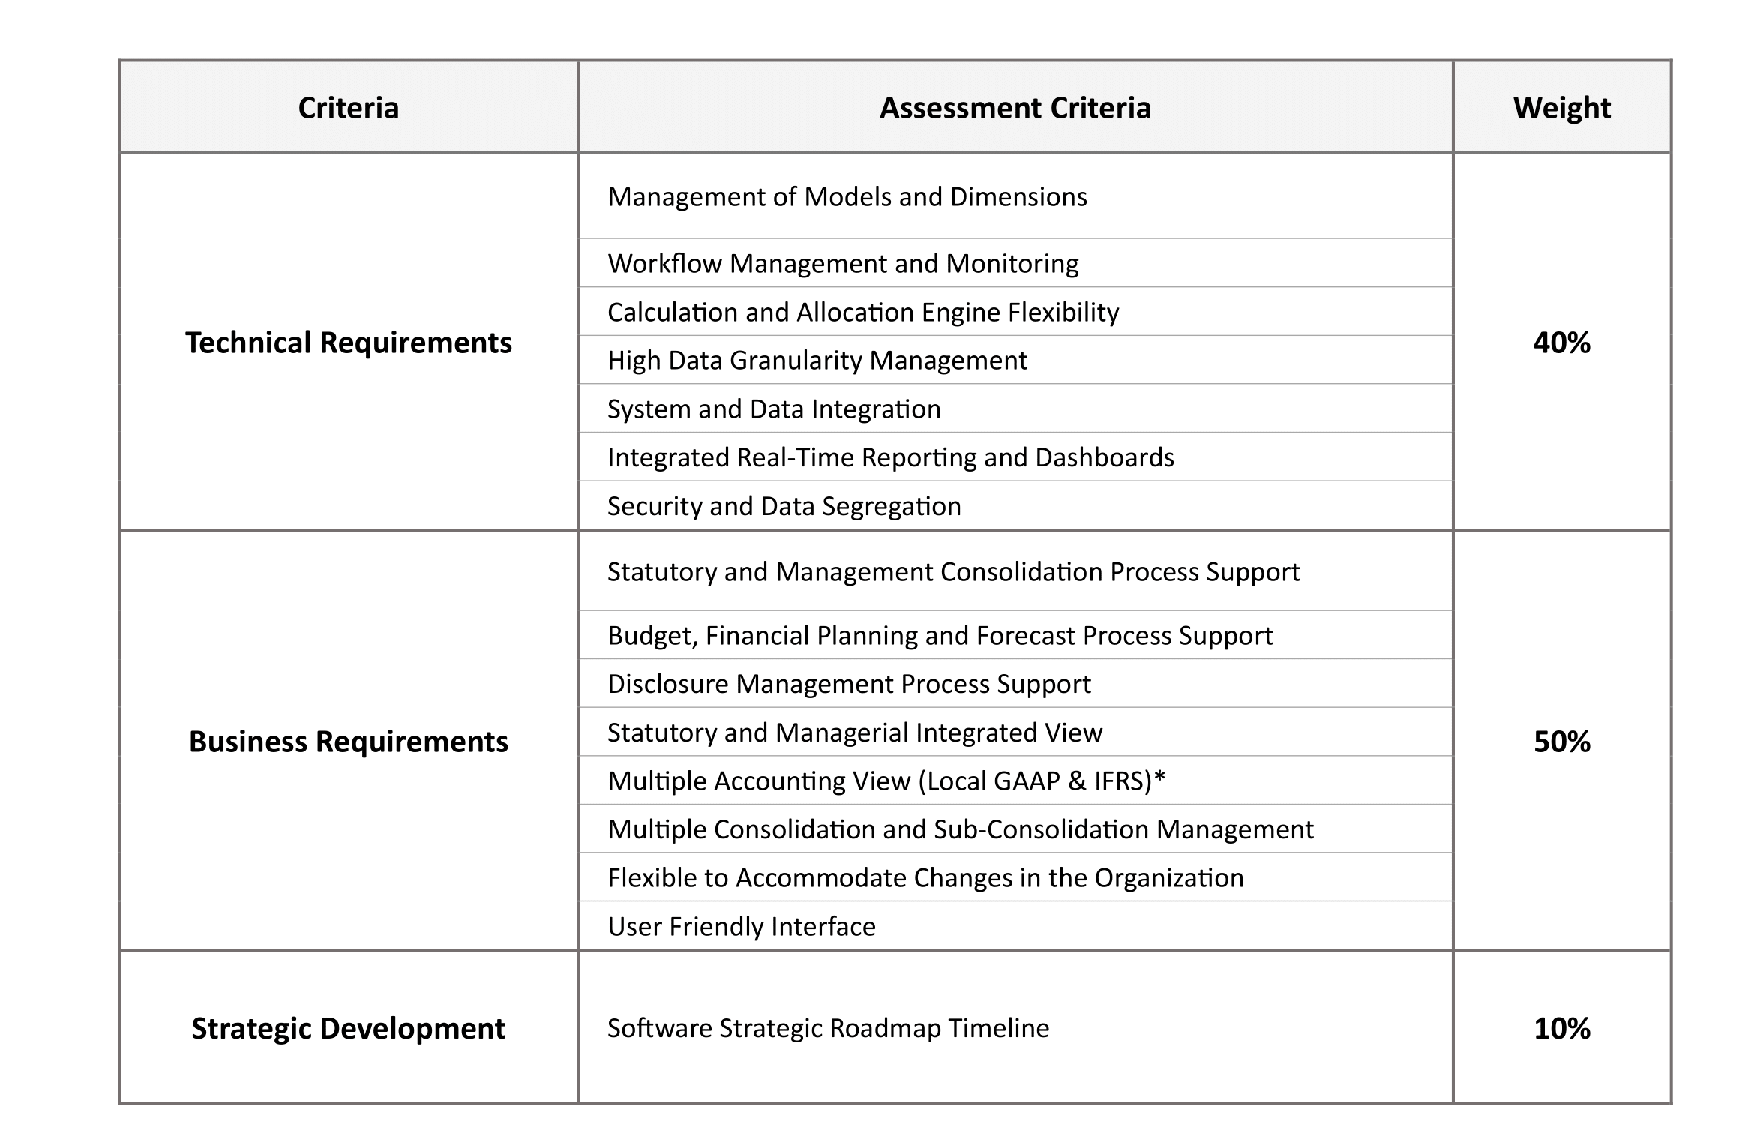
\includegraphics[width=\linewidth]{figures/requirements.pdf}
	\caption{Technical, Business and Strategic Requirements}
    \floatfoot{*Generally Accepted Accounting Principles (GAAP) and International Financial Reporting Standards (IFRS)}
	\label{fig:requirements}
\end{figure}

Figure \ref{fig:requirements} lists all the technical, business and strategic requirements that should be considered when choosing the right tools and technologies for the implementation of the EPM solution.
%
It is important to identify and prioritize both business requirements and technical requirements when planning an EPM implementation project, in order to build an effective and maintainable solution.

Technical requirements cover the specific features and capabilities that the system must have in order to ensure that the EPM system is effective, reliable, and able to meet the unique needs of the Holding Group and its Entities.
%
More in details, the use of technologies that allow for integrated modeling that is easy-to-maintain and with no limitations of dimensions is of key importance for this project.
%
For example, a Holding Group which owns different Brands and Entities across the globe may need to frequently update the \textit{Product} or \textit{Geography} dimension every time they add a new product or sell to a new country.
%
At the same time, users need to have a clear and structured workflow of activities that supports them in the use of the EPM system, while the Management Control Department should be able to track and monitor the progress of single activities carried out by the Entities.
%
Then, in terms of calculation and allocation flexibility, we refer to the possibility to perform custom calculations and extend predefined rules (like consolidation and currency translation), in order to meet the specific needs and requirements of each Entity.
%
The system should also be able to manage data of different granularity as the level of detail and precision in data structures depends on the activity to perform.
%
The EPM platform needs to manage high-volume data and possibly interface with big data systems.
%
Naturally, system and data integration must be available.
%
In particular, the system should have an integrated solution for ETL (Extract, Transform and Load) activities, completed with advanced mapping features to accommodate multi-source and multi-ERP loading.
%
Reporting and dashboarding can be setup ``live'' for all data available in the interconnected solution
applications to enable the Holding Group to make informed decisions based on its financial data.
%
Finally, the EPM system should have robust security features to protect sensitive financial data, while allowing the Management Control Department to manage granular securities at the micro-detail of data to handle the read and write permissions of the different entities.

Business requirements, on the other hand, regard the specific goals, needs, and expectations of the stakeholders and users of a system. 
%
In our context of EPM implementation project for a Holding Group, business requirements are set to reach key business goals, like streamlining financial reporting, improving decision-making based on financial data, increasing efficiency and accuracy in budgeting and forecasting, and providing a centralized system for financial management across all entities. 
%
One of the key priorities for a Holding Group is to have a clear statutory and consolidation process with the possibility to adopt multiple consolidation methods, including full consolidation, proportionate consolidation, and equity consolidation.
%
Consolidation accounting is the process of combining the financial results of several subsidiary companies into the combined financial results of the parent company as though they were a single firm.
%
The system should have predefined modules to address different planning standard processes and an open ``free from'' planning mode to create personalized planning environments. 
%
At the same time, it should include embedded predictive planning, risk based planning and strategic  long-term modeling feature.

Public companies must prepare disclosure reports for internal and external stakeholders to shine a light on the company's performance and operating activities.
%
Disclosure reports contain information about a company's business activities, financial condition, management compensation, operating performance and future direction. 
%
It is therefore essential for the EPM system to provide disclosure management functionalities to help the Holding Group to fulfill the disclosure requirements of regulators like the Security and Exchange Commission or the European Central Bank.
%
The system should provide  a unified environment able to guarantee the consistency and coherence of data generated at each level of the statutory, management and disclosure reporting.
%
In this regard, users should be able to compare multiple accounting views depending on the country of interest (GAAP for United States and IFRS world-wide).
%
Finally, the EPM system should be flexible enough to adapt to changing business needs and requirements, allowing for an easy-to-use, adjustable interface that every user can use to create different versions of reports, depending on the current need.

At the strategic level, making architecture changes or modifying operations takes a clear plan of where the organization is, where it wants to go, and how to get there. 
%
A strategic road-map lays out the direction of IT efforts that span across an organization in a simple way to align teams and key stakeholders.
%
The implementation of the EPM solution should be in line with the company's strategic road-map, both in terms of deliverables, process schedule and timing.

\section{Overview of the methodology}

The successful implementation of an Enterprise Performance Management system can have a significant impact on the performance and competitiveness of a business. 
%
However, the implementation of such a system requires careful planning, preparation, and execution to ensure success. 
%
In this section, we will examine the methodology used in the implementation of a Oracle Cloud EPM solution for the Holding Group.
%
We will explore specific approaches, methodologies, and tools used in each phase of the project, and discuss the challenges and lessons learned throughout the implementation. 
%
By examining the methodology used in this project, we can gain insights into best practices for Oracle Cloud EPM implementation and its unique features and tools.
%
The methodology applied to the implementation of an Enterprise Project Management solution follows some key steps and best practices that depend on the specific requirements of the company, the size and complexity of the project and the available resources.
%
The entire implementation process is built together with the Management Control Department of the Holding Group, which is responsible for assessing the quality of each step and ensuring the compliance with the requested features of the system.

The project begins with a planning phase, during which the company's business needs and goals are identified and the scope of the project is defined.
%
This involves identifying the objectives and key deliverables of the project, as well as any constraints or assumptions that will impact the implementation.
%
During this phases, it is important to identify the stakeholders by determining who will be impacted by the implementation and what their needs and requirements are.
%
A project plan is a comprehensive document that outlines the key objectives, milestones, tasks, timelines, and resources required for the successful completion of a project. 
%
It is an essential tool for project management, as it provides a road-map for project execution and allows for effective tracking and monitoring of progress.
%
Project plans help to define the scope and objectives of the project, identify the specific tasks and activities required to achieve the project objectives and determine the timelines and milestones for each task and activity.
%
At an operational level, designing a precise project plan allow for the effective allocation of the necessary resources, such as budget, personnel, and equipment, to complete the project.
%
At the same time, it ensure effective communication and collaboration between team members while facilitating the tracking and monitoring of progress towards project goals.
%
It gives a good reality check and enables to change course if needed, bringing the project back on track. 
%
Finally, during this planning phase, the definition of success criteria is performed, in order to measure the outcome by using performance indicators.

Along the planning phase, it is essential to conduct a needs assessment to efficiently allocate resources and set the details for the solution design.
%
The needs assessment is a systematic process for determining and addressing needs and requirements to fill the gap between the current conditions and the desired conditions.
%
The goal of this initial phase is to assess the current financial reporting and analysis process used by the Holding Group to identify pain points, inefficiencies and areas of improvement.
%
The key steps carried out during the process, include:

\begin{enumerate}
    \item Identification of the requirements: understanding everything that is involved with the project, ensuring that the project’s context and objectives are clear. By understanding the specifics, it is easier to identify the needs associated with the project, as well as explaining individual milestones and deliverables to the people involved to provide a broader context.
    \item Selection of the resources: match the existing, available resources to what is needed to perform the project. 
    \item Identification of potential gaps: once the resources have been identified, we can truly address the ones that are not already fulfilled. In this way, we will make sure to uncover and address any gaps, which can vary from a particular skill set to the software needed to execute a task. 
    \item Creation of a plan to fill the gaps: once all the gaps have been successfully identified, we can use this information and address these issues by designing a plan of action. 
\end{enumerate}

Overall, the needs assessment phase is critical in ensuring that a project is aligned with the needs of its intended beneficiaries, and that it is designed to meet their needs and address the specific problem or opportunity effectively.

Now that we have a clear plan for the implementation process, we can design the EPM solution based on the identified business requirements and goals.
%
Solution design involves translating the gathered requirements into a detailed design for the Oracle Cloud EPM solution. 
%
The solution design process encompasses various aspects, such as the system configuration, to configure the Oracle Cloud EPM environment based on the requirements, the workflow design and the reporting design, to meet the Holding Group's reporting needs.
%
The implementation phase involves deploying the designed solution while continuously assessing and refining the system. 
%
This include the monitoring and evaluatioon of the implemented solution during the User Acceptance Testing (UAT), to gather feedback and identify areas for improvement or modifications. 

Once the solution is live, ongoing support and training are crucial. 
%
User training programs are conducted to ensure users understand how to effectively use the Oracle Cloud EPM systems.
%
At the same time, it is important to regularly implement system enhancements and upgrades to keep the solution up-to-date.
%
Additionally, user adoption and change management strategies are employed to promote the use of the EPM solution throughout the organization. 
%
This involves monitoring user feedback, measuring system usage, and implementing change management practices to ensure a smooth transition and alignment with the implemented solution.

%----------------------------------------------------------------------------------------
\chapter{Enterprise Performance Management}
\label{chap:epm}
%----------------------------------------------------------------------------------------

In today's dynamic and highly competitive business landscape, organizations face numerous challenges in effectively managing and improving their performance. 
%
One of the monitored outputs of being able to thrive among rivals in turbulent markets is to excel at various performance dimensions. 
%
One of the prerequisites for this is to be able to effectively manage and measure corporate performance using various performance management and measurement systems.
%
Enterprise Performance Management has emerged as a critical discipline that enables businesses to align their strategies, measure their performance, and make informed decisions to achieve their goals. 
%
As organizations increasingly turn to cloud-based solutions to enhance their operational efficiency, Oracle Cloud EPM has emerged as a leading platform in this domain.

This chapter presents a comprehensive literature review that explores the theoretical foundations, best practices, and advancements in Enterprise Performance Management, with a specific focus on Oracle Cloud EPM. 
%
This review aims at providing valuable insights and a solid understanding of the concepts, methodologies, and technologies that drive effective performance management in today's digital era. \\

Over the years, Enterprise Performance Management has evolved from traditional financial-centric approaches to a more holistic and integrated framework that encompasses financial, operational, and strategic aspects of performance management. 
%
It has moved beyond mere financial reporting and budgeting to encompass performance measurement, analysis, forecasting, and decision support across all functional areas of an organization.
%
Moreover, the digital revolution has significantly impacted the evolution of EPM. 
%
The availability of vast amounts of data, advancements in data analytics, and the proliferation of cloud computing have transformed how organizations collect, analyze, and utilize performance-related information.

In a 2021 press release, KPMG\footnote{KPMG is one of the leading global professional services firms, providing audit, tax, and advisory services to organizations across various industries. Known for its extensive knowledge in areas such as financial reporting, risk management, and business transformation, KPMG plays a significant role in shaping the business landscape and driving innovation.} outlined how enterprise performance management has evolved as a result of the post-pandemic landscape, presenting new opportunities for organizations \cite{kpmg2021evolution}.
%
In the midst of the ongoing pandemic, organizations were grappling with unprecedented levels of uncertainty that had disrupted business operations and strategies. 
%
As the future remains uncertain, the survival and success of most organizations now hinge on their ability to engage in effective scenario planning.
%
Scenario planning relies heavily on accurate and reliable data to develop realistic plans, budgets, and forecasts. 
%
Organizations must establish robust data governance frameworks that ensure the availability of good-quality internal and external data. 
%
At the same time, with rapidly changing circumstances, organizations need to adopt a dynamic approach to planning and forecasting to respond effectively to evolving situations. 
%
Embracing scenario planning allows organizations to explore various potential future outcomes, develop resilient strategies, and gain a competitive edge: as uncertainties persist, organizations that prioritize scenario planning will be better equipped to thrive in changing circumstances and emerge stronger in the long run.

In the present era, Enterprise Performance Management has undergone significant evolution. 
%
Despite the advancements in modern analytics and business intelligence, a considerable 54\% of finance organizations still encounter challenges in providing data that effectively supports stakeholders' decision-making. \cite{gartner2021report}
%
Often, the insights generated lack contextual information and are not easily comprehensible for the majority of users who primarily engage with pre-defined dashboards. 
%
Furthermore, certain organizations continue to rely on outdated systems, and the budgeting process can still consume up to four months to reach completion.
%
On a global scale, organizations that have embarked on their EPM journey have strategically shifted their focus from reactive and descriptive reporting to proactive and forward-looking prescriptive analysis. 
%
By devoting more time to providing forward-looking guidance, management can effectively capitalize on upcoming opportunities and gain more meaningful insights to support superior decision-making. 
%
This transformation can be achieved by harnessing the power of predictive and prescriptive analytics techniques, which enable organizations to anticipate future outcomes and prescribe optimal courses of action.

\section{Definition and concepts}

Enterprise Performance Management (EPM) is a comprehensive approach that helps organizations effectively manage and optimize their performance in order to achieve strategic goals and objectives. 
%
It involves the systematic measurement, analysis, and improvement of key performance indicators (KPIs) across various business functions and levels of the organization.
%
With EPM software, companies can align business strategy with business execution. 
%
The technology uses feedback drawn from data generated from systems, processes, and activities across the organization. 
%
The resulting analytics help to identify business drivers and other insights so that companies can assess new opportunities, augment profitability in existing business, and respond with greater agility in the face of unexpected change and disruption.

Neely et al. \cite{neely2002performance} define a performance measurement system as a ``set of metrics used to quantify the efficiency and effectiveness of past actions'' that ``enables informed decisions to be made and actions to be taken because it quantifies the efficiency and effectiveness of past actions through the acquisition, collation, sorting, analysis and interpretation of appropriate data.''
%
The geographical location of a firm, historical development of a country/region and an enterprise culture have played significant roles in reinventing performance management systems. 
%
Nowadays, effective systems explicitly address not only economic trends but also social, political and environmental ones.

\begin{figure}[h]
	\centering
	\includegraphics[]{figures/cycle.pdf}
	\caption{Enterprise Performance Management Framework}
    \floatfoot{Source: PricewaterhouseCoopers HK}
	\label{fig:cycle}
\end{figure}

Figure \ref{fig:cycle} represents the three main stages of Enterprise Performance Management, each of which plays a critical role in managing and improving the performance of a business. 
%
The strategy phase is the foundation of the EPM cycle, where the business establishes its objectives and formulates its strategic plans. 
%
This phase involves the following key activities: objective setting, planning and budgeting.
%
Firstly, the business defines its short-term and long-term objectives, which could include revenue targets, market share goals, cost reduction objectives or customer satisfaction metrics.
%
Then, based on the objectives, the business develops a comprehensive plan to achieve its goals by identifying key initiatives, allocating resources, and setting timelines.
%
Finally, the business drafts a budget with the aim of allocating financial resources to different departments, projects or activities, ensuring that the financial plans align with the strategic objectives.
%
The outcome of the strategy phase is a well-defined roadmap that guides the organization's actions in the subsequent stages of the EPM cycle.

Then, the execution phase focuses on implementing the plans and strategies developed in the strategy phase and involves activities related to reporting, control, and performance tracking.
%
The business collects and analyzes data from various sources, such as financial and operational systems and then transform the data collected into meaningful reports and dashboards that provide insights into the organization's performance.
%
At the same time, through an attentive control process, the business makes sure that the defined plans and objectives are followed by monitoring key metrics, comparing actual results against targets, and taking corrective actions when necessary.
%
The execution phase is crucial for ensuring that day-to-day activities are aligned with the overall goals of the business.

Finally, the performance phase involves evaluating the organization's performance, calculating key performance indicators (KPIs), and deriving insights to drive continuous improvement. 
%
This is done by assessing the business performance against the objectives set in the strategy phase and by calculating KPIs to measure the organization's progress on an operational and strategical level.
%
The insights gained from performance evaluation and KPI analysis guide decision-making processes, helping identifying areas of strength, areas for improvement, and potential opportunities for growth.

As the business world is continuously changing, performance management systems are continuously remastered and updated to maintain their effectiveness.
%
Top performers studied by The Hackett Group\footnote{The Hackett Group is a leading global consulting firm that specializes in business performance improvement and benchmarking. Founded in 1991, The Hackett Group offers a wide range of advisory services, research, and best practice insights to help organizations optimize their operations, enhance efficiency, and achieve world-class performance.} have recognized the importance of aggressively reducing Enterprise Performance Management complexity while simultaneously embracing new waves of digital capability.
%
These organizations understand that simplifying and streamlining their EPM processes and systems can lead to improved efficiency, agility, and improved decision-making. \cite{balog2017best}
%
EPM complexity refers to the intricate set of processes, systems, and data that can often burden organizations and hinder their ability to effectively manage performance. 
%
Complex EPM environments are characterized by fragmented data sources, manual data collection and consolidation, siloed planning and reporting processes, and a lack of integration between different EPM components. 
%
Such complexity can result in inefficiencies, data inconsistencies, and delays in decision-making, ultimately impacting an organization's ability to achieve its strategic goals.
%
By simplifying the EPM landscape, businesses can eliminate redundancies, streamline processes, and reduce the time and effort required to collect, analyze, and report on performance data. 
%
This simplification allows organizations to focus on value-added activities, such as analysis, forecasting, and strategy execution.
%
At the same time, by leveraging emerging technologies, such as advanced analytics, artificial intelligence, machine learning and automation, organizations can gain greater insights into their business operations and identify patterns and trends in data.
%
However, it is essential to note that while reducing complexity and embracing digital capability are critical, organizations must also ensure a careful balance between simplicity and meeting the specific needs and complexities of their business. The approach should be tailored to their unique requirements, considering factors such as industry dynamics, organizational structure, and regulatory compliance.

Enterprise Performance Management is continuously evolving as organizations seek innovative approaches to improve their performance and achieve strategic objectives. 
%
In this era of rapid technological advancements, emerging technologies such as Big Data and the Internet of Things (IoT) have emerged as powerful enablers for driving sustainable practices and enhancing EPM. 
%
By leveraging the capabilities of these technologies, organizations can gain deeper insights into their environmental impact, social responsibility, and economic sustainability. \cite{yang2023bigdata}
%
The combination of these new technologies enables organizations to gather and analyze vast amounts of real-time data from various sources, leading to more accurate and comprehensive insights into their performance.
%
While the integration of Big Data and IoT in EPM brings about significant advantages, it also presents its share of challenges. 
%
Organizations must navigate issues related to data privacy, data quality, data integration, and technological infrastructure and need to develop robust data governance frameworks to ensure security and integrity for the data collected. 
%
Additionally, organizations must invest in the necessary technology infrastructure and analytical capabilities to effectively manage and derive value from the vast amounts of data generated by IoT devices and other sources.

As we have seen, Enterprise Performance Management plays a crucial role in helping organizations effectively manage their performance and achieve strategic objectives. 
%
In today's data-driven world, the integration of Business Intelligence (BI) tools and techniques within EPM has become essential for organizations to gain valuable insights and make informed decisions. 
%
Stefan et al. \cite{stefan2010enterprise} provide a comprehensive approach to develop a decision-performance relationship within a company by identifying key factors and performance indicators. 
%
They emphasize the importance of integrating performance evaluation not only at the individual employee level but also within project teams and the overall organizational performance. 
%
The premise of this approach is that performance evaluation should be viewed holistically, taking into account the interdependencies and collaboration among employees, teams, and the organization as a whole.
%
One of the fundamental aspects highlighted in the paper is the need for a continuous flow of monitoring and analysis to build a sustainable mechanism for supporting organizational performance. 
%
This aligns with the core principles of EPM, which emphasize the importance of ongoing measurement, analysis, and improvement of key performance indicators, making the integration of Business Intelligence within EPM an opportunity to unlock the full potential of their performance data. 

\section{Benefits and challenges of implementing EPM in businesses}

As organizations strive for excellence, EPM offers a systematic approach to measuring, managing, and improving performance across various dimensions. 
%
By integrating financial, operational, and strategic aspects, EPM enables businesses to gain a holistic understanding of their performance and make data-driven decisions to achieve their goals. 
%
However, the implementation of EPM is not without challenges and organizations must navigate potential hurdles to maximize the benefits it offers.
%
This section explores the benefits and challenges associated with the implementation of EPM, shedding light on how it can drive organizational success while also acknowledging the complexities involved.

In terms of benefits, EPM provides organizations with several advantages. 
%
First and foremost, it facilitates improved performance measurement and reporting: by establishing clear performance indicators and metrics, organizations can track progress, identify areas of strength and weakness, and align their efforts towards continuous improvement. 
%
EPM also enhances transparency and accountability, enabling stakeholders to access accurate and timely performance information, fostering trust and facilitating effective communication.
%
Another benefit of EPM is its ability to support strategic alignment. 
%
By integrating performance management with strategic objectives, organizations can ensure that day-to-day activities align with long-term goals. 
%
This alignment enhances decision-making at all levels of the organization, enabling employees to understand how their work contributes to overall success and fostering a culture of accountability and empowerment.
%
EPM also enables organizations to leverage data and analytics for better insights and decision-making to identify opportunities, mitigate risks, and make proactive decisions based on real-time information.

Despite the numerous benefits, implementing EPM can pose challenges for organizations. 
%
Common hurdles include resistance to change, resource constraints, and the need for a robust technology infrastructure. 
%
Successful implementation requires buy-in from stakeholders, effective change management strategies, and the allocation of appropriate resources to support the EPM initiatives. 
%
Furthermore, organizations must navigate complexities related to data integration, data quality, and ensuring the security and privacy of sensitive information.

Organizations that have implemented Enterprise Performance Management have reaped significant benefits, as highlighted by two key findings. 
%
The first finding, derived from a press release issued by Oracle Corporation in 2022 \cite{toomey2022oracle}, reveals that Oracle Cloud EPM customers have experienced a remarkable 61\% improvement in forecast accuracy. 
%
This improvement is a testament to the power of EPM in providing organizations with better visibility and control over their financial planning processes. 
%
By leveraging EPM solutions, organizations can align their financial plans with other critical areas such as supply chain, sales, project, and workforce planning. 
%
This integration enables a more holistic and comprehensive approach to decision-making, ultimately driving improved forecast accuracy and facilitating better-informed strategic choices.
%
The second finding, derived from KPMG's 2021 EPM survey \cite{kpmg2021survey}, underscores the positive impact of EPM on revenue growth. 
%
According to the survey, 72\% of mature EPM clients have already embarked on their EPM journey, actively embracing EPM practices such as supporting centers of excellence, predictive forecasting, and upskilling their employees. 
%
These organizations have witnessed a remarkable 20\% increase in revenue over the past three years. 
%
This finding highlights the transformative potential of EPM in driving financial performance and business growth. 
%
By implementing EPM methodologies, organizations can establish a culture of excellence, empower employees with advanced forecasting and analytical capabilities, and optimize their financial planning and decision-making processes. 
%
The result is enhanced revenue generation and improved financial outcomes.

These findings collectively demonstrate the tangible benefits that organizations can achieve through the successful implementation of EPM. 
%
Improved forecast accuracy ensures more reliable financial planning, enabling organizations to make better-informed decisions and adapt to market dynamics effectively. 
%
Furthermore, revenue growth serves as a clear indicator of the positive impact that EPM can have on overall business performance. 
%
By embracing EPM practices and leveraging advanced technologies, organizations can unlock their full potential, align their operations, and drive sustainable growth.
%
It is important to note that these benefits are not automatic, and organizations must navigate challenges associated with EPM implementation, including change management, resource allocation, and technology infrastructure. 
%
However, the rewards, as evidenced by the findings, are substantial. 
%
Organizations that invest in EPM, establish a robust EPM framework, and prioritize continuous improvement and upskilling initiatives stand to gain a competitive advantage in today's rapidly evolving business landscape. 
%
These findings underscore the value of EPM as a strategic enabler, empowering organizations to drive accurate forecasts, align financial plans with other critical areas, and ultimately achieve revenue growth and financial success.

%----------------------------------------------------------------------------------------
\chapter{Oracle Cloud EPM Implementation}
\label{chap:implementation}
%----------------------------------------------------------------------------------------

In this chapter we will explore the case study of an Oracle Cloud EPM implementation project for an international Holding Group with multiple entities.
%
Such implementation was necessary for the Holding Group to streamline financial reporting, improve decision-making based on financial data and, most importantly, provide a centralized system for financial management across all entities.

The Holding Group has a complex financial structure and was facing significant challenges in managing financial data across all entities. 
%
Its financial systems were disconnected, making it difficult to get a clear view of financial performance and to generate accurate and timely reports. 
%
In addition, its reporting processes were inefficient, relying heavily on manual data entry and resulting in errors and inconsistencies. 
%
Also, they lacked visibility into financial data across all entities, making it difficult to make informed decisions and to drive growth and profitability.

Throughout this case study, we will examine each step of the implementation process, analyzing the structure of the EPM solution and the data load process.
%
We will start by defining the solution selection process, moving to the structure of the solution and then, we will examine in depth the implementation phase.

\section{EPM solution selection}

Selecting the right EPM solution is crucial to effectively manage the financial data of the Holding Group and drive growth.
%
In order to design a solution architecture for consolidation, planning and reporting that is able to provide system integration, automatic and standard processes, we need to identify the most suitable EPM tool among the ones available in the market.

\begin{figure}[htbp]
	\centering
	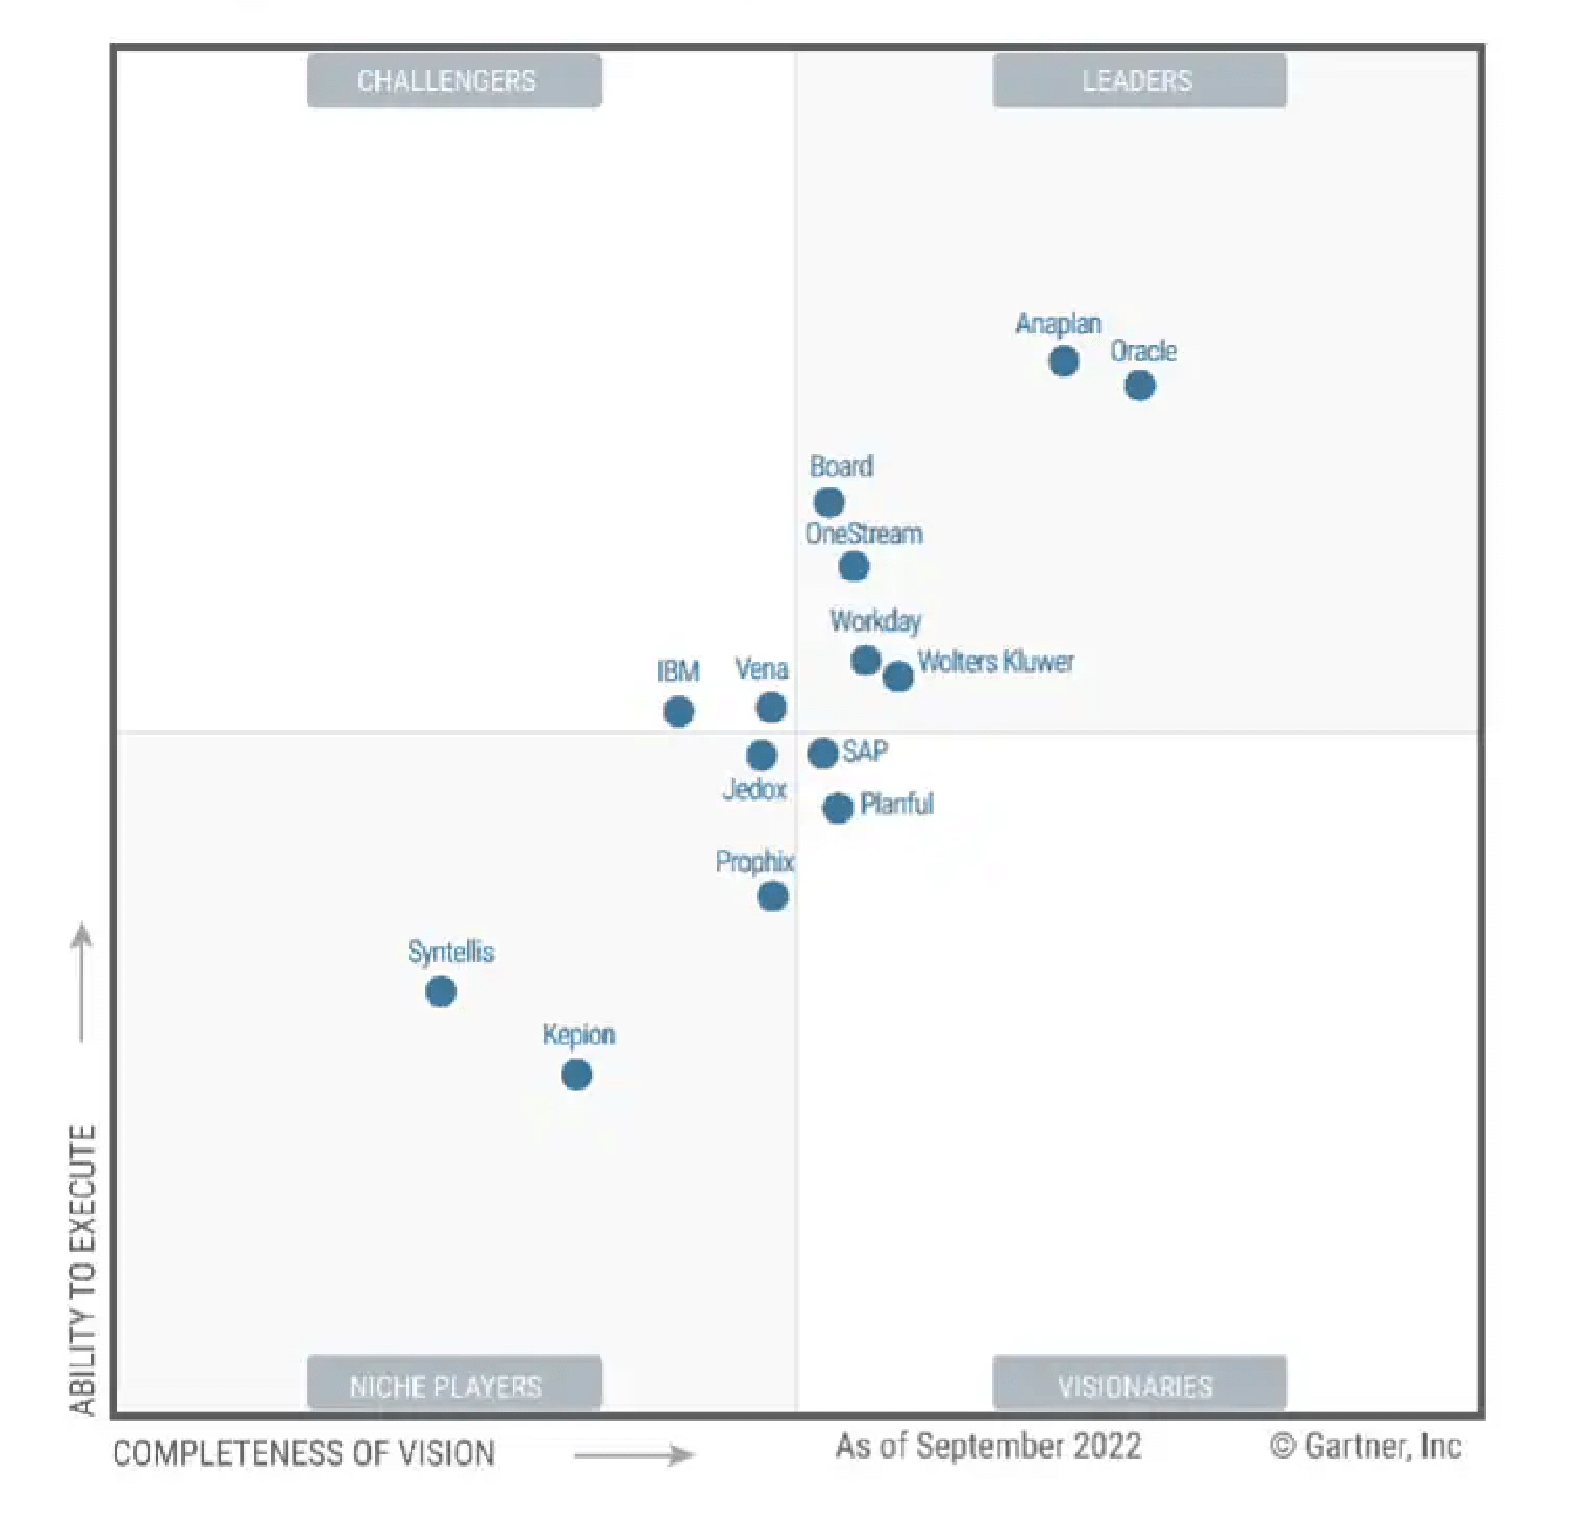
\includegraphics[width=\linewidth]{figures/gartner.pdf}
	\caption{Magic Quadrant for Financial Planning Software}
    \floatfoot{Source: Gartner (December 2022)}
	\label{fig:gartner}
\end{figure}

Figure \ref{fig:gartner} displays the Gartner Magic Quadrant for financial planning software published on the 14th December, 2022 \cite{gartner2022magic}.
%
Gartner defines Financial Planning Software as ``the key tool that enables organizations to manage their enterprise-wide financial planning, forecasting, and budgeting processes.'' \footnote{Gartner is a registered trademark and service mark and Magic Quadrant is a registered trademark of Gartner, Inc. and/or its affiliates in the U.S. and internationally and are used herein with permission. All rights reserved.}

Financial Planning Software solutions allow organizations to plan and analyze the business financial strategy across all three financial statements (profit and loss, balance sheet, and cash flows). 
%
It supports modeling, collaboration, analytics, and performance-reporting capabilities, all of which enhance a user’s ability to effectively manage financial performance.
%
The Magic Quadrant evaluates vendors based on their completeness of vision and ability to execute. 
%
Oracle Cloud has been named a Leader in the Gartner Magic Quadrant for Cloud Financial Planning and Analysis Solutions for several years in a row. 
%
This recognition highlights Oracle's continued commitment to innovation and customer satisfaction. 
%
As a Leader in the Magic Quadrant, Oracle Cloud is recognized for its ability to provide a comprehensive and customizable EPM solution for Holding Groups and other organizations.

According to Oracle Corporation, the current global uncertainties have proven the value of Oracle Fusion Cloud EPM as businesses of every size have experienced extreme volatility in demand and supply environments, making agility in financial planning processes a must-have competency \cite{toomey2022oracle}.
%
The ability to support and connect planning across the organization is a competitive differentiator. 
%
Oracle delivers purpose-built solutions to streamline and manage planning processes in sales, marketing, human resources, IT and supply chain functions.
%
Oracle Cloud EPM brings together multiple Enterprise Performance Management capabilities into a single suite: financial and operational planning, profitability and cost management, account reconciliation, consolidation and close, tax reporting, narrative reporting, and enterprise master data management. 
%
These capabilities, along with built-in best practices, help customers to gain value quickly.

For the Holding Group in our case study, Oracle Cloud EPM was the right choice due to its ability to be customized to meet the specific needs of the organization, its comprehensive security and compliance features, and its strong support and training resources.
%
Choosing the right EPM solution can make all the difference in the Holding Group's ability to effectively manage their financial data and drive growth and profitability.

\section{Elements of the implementation process}

To successfully implement a new system, it is essential to have a comprehensive understanding of the various elements that are involved in the process. 
%
This section explores the essential elements necessary for a successful EPM implementation process, providing a roadmap for organizations seeking to deploy EPM solutions effectively.
%
Throughout this section, we will delve into key components that form the foundation of an EPM implementation solution. 

\paragraph{License}

Oracle Cloud Enterprise Performance Management is a complete and connected EPM solution which, with one licensing subscription, gives access to planning, close and consolidation, account reconciliation, narrative reporting, and more.
%
Users can access all these models with their license; they do not need a license for each model.
%
There are two types of licenses according to which specific functionalities and features for users are enabled within the application:
%
The user-based licenses are assigned to individual users who require access to the application.
%
These licenses provide access to specific functionalities within the application, and the features available to each user may vary based on the license type and configuration.
%
On the other hand, instance-based licenses are allocated to the overall EPM environment, rather than individual users. 
%
These licenses are typically purchased in bundles and may be allocated based on factors such as the number of users or the level of usage.
%
Oracle will provision by default two environments to users: one environment dedicated to production use and a second environment dedicated as a staging environment for non-production use.
%
Additional environments or business processes can be ordered and provisioned separately.

\paragraph{Environments}

Oracle Cloud EPM applications are typically deployed in two environments: production and test.
%
The production environment is the live environment where users interact with the EPM application to perform their day-to-day financial management tasks.
%
The test environment, on the other hand, is a sandbox environment in which we can test new features, perform system upgrades, and make changes without affecting the live production environment. 
%
Both the environments can be accessed via unique launch URLs composed by the service name (EPM), the type of environment (test or production), the identity domain name and the data center in which the environment is located.\\

\begin{lstlisting}[
    basicstyle=\footnotesize
    ]
https://epm-idDomain.epm.dataCenterRegion.oraclecloud.com/epmcloud
\end{lstlisting}

\paragraph{Modules and Applications}

The suite of Oracle Cloud EPM includes various modules that are designed to address specific business needs:
%
Planning and Budgeting enables organizations to streamline their budgeting and forecasting processes, allowing for collaboration across teams, flexible modeling, and real-time updates to data.
%
Financial Consolidation and Close automates the financial consolidation and close process, helping organizations to reduce errors and improve accuracy, providing a standardized approach to the close process and supporting compliance with regulatory requirements.
%
Account Reconciliation streamlines the account reconciliation process, helping organizations to reduce risk and improve accuracy. 
%
Profitability and Cost Management enables organizations to gain insights into their profitability and cost structures, supporting activity-based costing, providing allocation and modeling capabilities and what-if analysis.
%
Enterprise Data Management provides a centralized platform for managing master data across the organization, supporting data governance and compliance, data quality management capabilities, and enabling seamless integration with other EPM modules.
%
Narrative Reporting enables organizations to create, manage, and distribute financial and management reports.
%
Tax Reporting supports compliance with tax regulations and provides a comprehensive solution for tax reporting, including a tax data warehouse, data validation and mapping capabilities, and supporting data visualization.
%
In this case study, we will see more in details the Planning and Budgeting application together with Oracle's Financial Consolidation and Close Solution (FCCS) and Enterprise Data Management.

\paragraph{Data Structure}

One of the core components of Oracle Cloud EPM is Essbase, which is multidimensional database management system (MDBMS) that enables businesses to store, manage, and analyze large volumes of data from different sources.
%
Multidimensional databases are specialized databases designed for online analytical processing (OLAP). 
%
They store data in a cube-like structure where each cell represents a specific data point.
%
Unlike relational databases, which store data in tables, multidimensional databases use a multidimensional model that allows users to analyze data across multiple dimensions, such as time, geography, and product. 
%
One of the key features of MDBs is their ability to perform OLAP, enabling users to drill down or roll up data along different dimensions, providing a more comprehensive view of the data. 
%
Compared to Relational Databases, multidimensional Databases are faster and more efficient when dealing with large volumes of data, even though they are less flexible than RDBs when it comes to data modeling, and require specialized tools and expertise to manage and maintain.

\paragraph{Data Management}

Data management refers to the process of integrating and managing data from various sources within the EPM environment. 
%
The process begins with integrating data from various sources, such as ERP systems, spreadsheets, or other databases. 
%
Oracle Cloud EPM provides tools to help users extract and integrate data from these sources and map them to the appropriate EPM application or service.
%
Once the data has been integrated into the EPM environment, it needs to be validated to ensure that it is accurate, complete, and consistent. 
%
After the data has been validated, it may need to be transformed to match the specific requirements of the EPM application or service using predefined mappings, calculations or custom scripts.
%
Finally, the data can be loaded into the EPM application into the appropriate data structures within the application, such as dimensions or cubes. 
%
Oracle Cloud EPM provides tools to automate the steps of data management,  helping organizations streamline their data management processes allowing for a faster data integration with improved data quality, greater efficiency and reduced error rate.

\paragraph{Dimensions}

In Oracle Cloud EPM, dimensions are a fundamental component of multidimensional data modeling. 
%
Dimensions provide a way to organize and analyze data in a multidimensional structure, allowing users to perform complex analysis along them. 
%
They are typically structured as hierarchies, with each level in the hierarchy representing a different level of detail. 
%
Members represent the values within each level of the hierarchy and can be associated with attributes such as descriptions or tags to provide additional context. 
%
Hierarchies provide the ability to roll up or drill down data to gain insights into different levels of detail. 
%
Through dimensions, it is possible to execute dynamic calculations to generate on-the-fly calculations at runtime, without requiring the user to manually enter the data. 
%
This enables users to create dynamic models that are more flexible and responsive to changing business needs.

As we can see in figure \ref{fig:hierarchy}, the time dimension follows a tree-like structure where each level in the hierarchy represents a different level of detail. 
%
Hierarchies allow users to organize data into a structure that is easy to understand and navigate it, by grouping related data points together and providing a way to analyze data at different levels of detail, from high-level summaries to more detailed views of individual data points.
%
In this dimension, data can be dynamically aggregated along the levels in order to see the results with different levels of granularity, i.e. monthly, quarterly or yearly.

\begin{figure}[htbp]
	\centering
	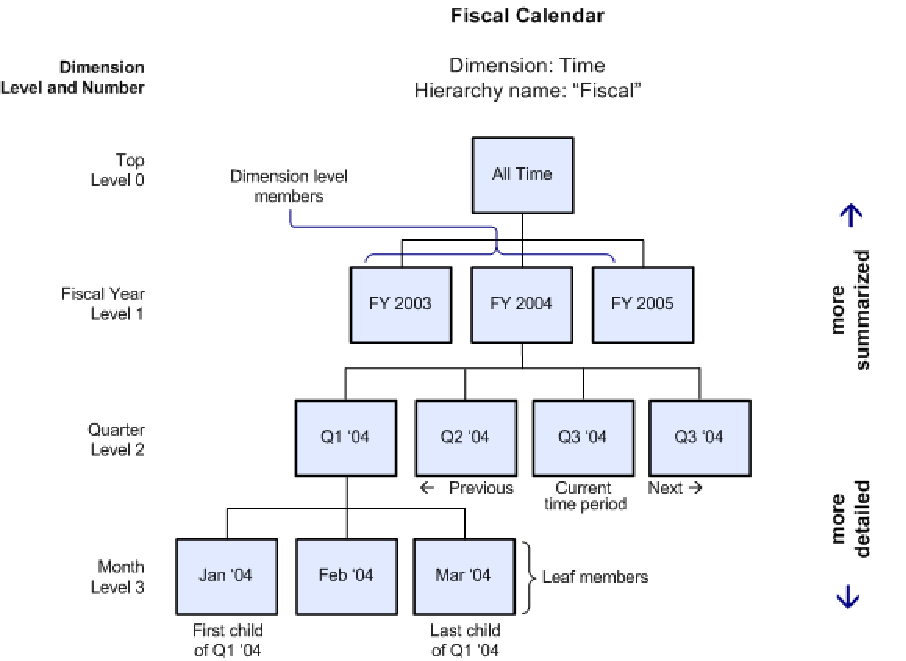
\includegraphics[width=\linewidth]{figures/hierarchy.pdf}
	\caption{Hierarchical Structure of the Time Dimension}
    \floatfoot{Source: Oracle User's Guide}
	\label{fig:hierarchy}
\end{figure}

\paragraph{Forms and Reports}

Forms and reports are key components of Oracle Cloud EPM that enable users to interact with and analyze data in a multidimensional database. 
%
Forms are used to input or edit data, while reports are used to analyze data in a structured format.
%
Forms provide users with a familiar interface for entering or editing data in a multidimensional database. 
%
They can be designed to incorporate a variety of data entry methods, including text boxes, drop-down lists, and radio buttons. 
%
Users can also navigate between different cells and dimensions in a form to enter or edit data in a specific location.
%
Reports, on the other hand, provide a way to analyze data in a structured format. 
%
These reports can be customized to include specific data points and dimensions, and can be designed to incorporate a variety of formatting options, including charts, graphs, and tables.
%
One of the key advantages of forms and reports is their flexibility. 
%
Users can design and customize forms and reports to meet their organization's unique business requirements, incorporating specific data points and dimensions as needed. 
%
This makes forms and reports a powerful tool for data analysis and decision-making.

\paragraph{Business Rules}

Business rules are a set of instructions that define how data should be calculated or transformed in a multidimensional database. 
%
These rules are used to automate complex calculations, validations, and transformations in a data model, reducing the need for manual data entry and increasing the accuracy of data analysis.
%
Business rules can be created using the Calculation Manager, which is the tool used to create, validate, deploy, and launch calculations in Oracle Cloud EPM. 
%
These rules can be based on various input data sources, including data entered manually, data loaded from external sources, or data calculated dynamically using other rules.
%
One of the key advantages of business rules is their flexibility: users can define rules that incorporate complex logic and are specific to their organization's unique business requirements. 
%
Rules can also be modified or updated easily as business needs change, making them a dynamic tool for data analysis.
%
%Oracle Planning offers powerful calculation features, including support for complex formulas, allocation rules, drivers, and multidimensional calculations. This enables organizations to perform sophisticated calculations while maintaining flexibility in their planning processes.


\paragraph{Smart View}

Smart View is an Excel add-in that allows users to connect to and interact with data in Oracle Cloud EPM. 
%
With Smart View, users can access dimensions, forms and reports directly from within Excel, enabling them to analyze and manipulate data in a familiar interface.
%
One of the key advantages of Smart View is its ability to integrate seamlessly with Excel. 
%
Users can work with data in Excel as they normally would, but with the added ability to access and manipulate data in a multidimensional database. 
%
This enables users to perform complex calculations and data analysis tasks using Excel's built-in functionality.
%
Smart View also provides a wide range of functionality beyond basic data access and manipulation. 
%
For example, users can use Smart View to create and manage ad-hoc reports, design custom templates for data entry and analysis, and build complex financial models using Excel's built-in functionality.
%
Another key advantage of Smart View is its ability to work with multiple data sources. 
%
Users can connect to and analyze data from a variety of sources, including Planning and Budgeting, Financial Close and Consolidation and more. 

\section{Building a comprehensive EPM solution}

The implementation of this EPM solution involves a systematic and comprehensive process which is aimed at ensuring accurate and comprehensive reporting to the user.
%
One crucial aspect of this process regards the creation of the dimensions that will be used to build reports from various perspectives. 
%
They are used to categorize and structure information in order to obtain a complete view on the performance of the Holding Group.

Dimensions are the building blocks of an EPM system; they serve as the axes along which data is organized and analyzed, providing a multidimensional view on financial and operational information. 
%
Each dimension consists of a hierarchical structure which allows users to drill down information from high-level summaries to more granular details and vice versa.
%
Dimensions serve several purposes, including analysis, reporting, data integration and restructuring.
%
First of all, dimensions allow for the segmentation and grouping of data which facilitate analysis and reporting by enabling users to generate reports based on specific dimensions, providing insights from different angles.
%
At the same time, they act as a common framework for integrating data from various sources within the Holding Group. 
%
Specifically, by aligning different systems and processes with a consistent set of dimensions, data can be harmonized and consolidated for accurate analysis and reporting.
%
Finally, dimensions provide flexibility to adapt to changing business requirements as they can be modified, expanded, or restructured to accommodate new entities, geographies, products, or brands as the Holding Group evolves.

Building dimensions require a systematic process during which different aspects are taken into account.
%
The first step is to analyze the specific needs of the Holding Group to identify the dimensions that will provide meaningful insights for analysis and reporting.
%
Then, it is essential to determine the levels of the hierarchy for each dimension and assign member properties to capture additional information about each dimension member. 
%
These properties provide contextual information and can include attributes such as currency, time zone, brand category, or legal Entity type. \\

\begin{figure}[htbp]
	\centering
	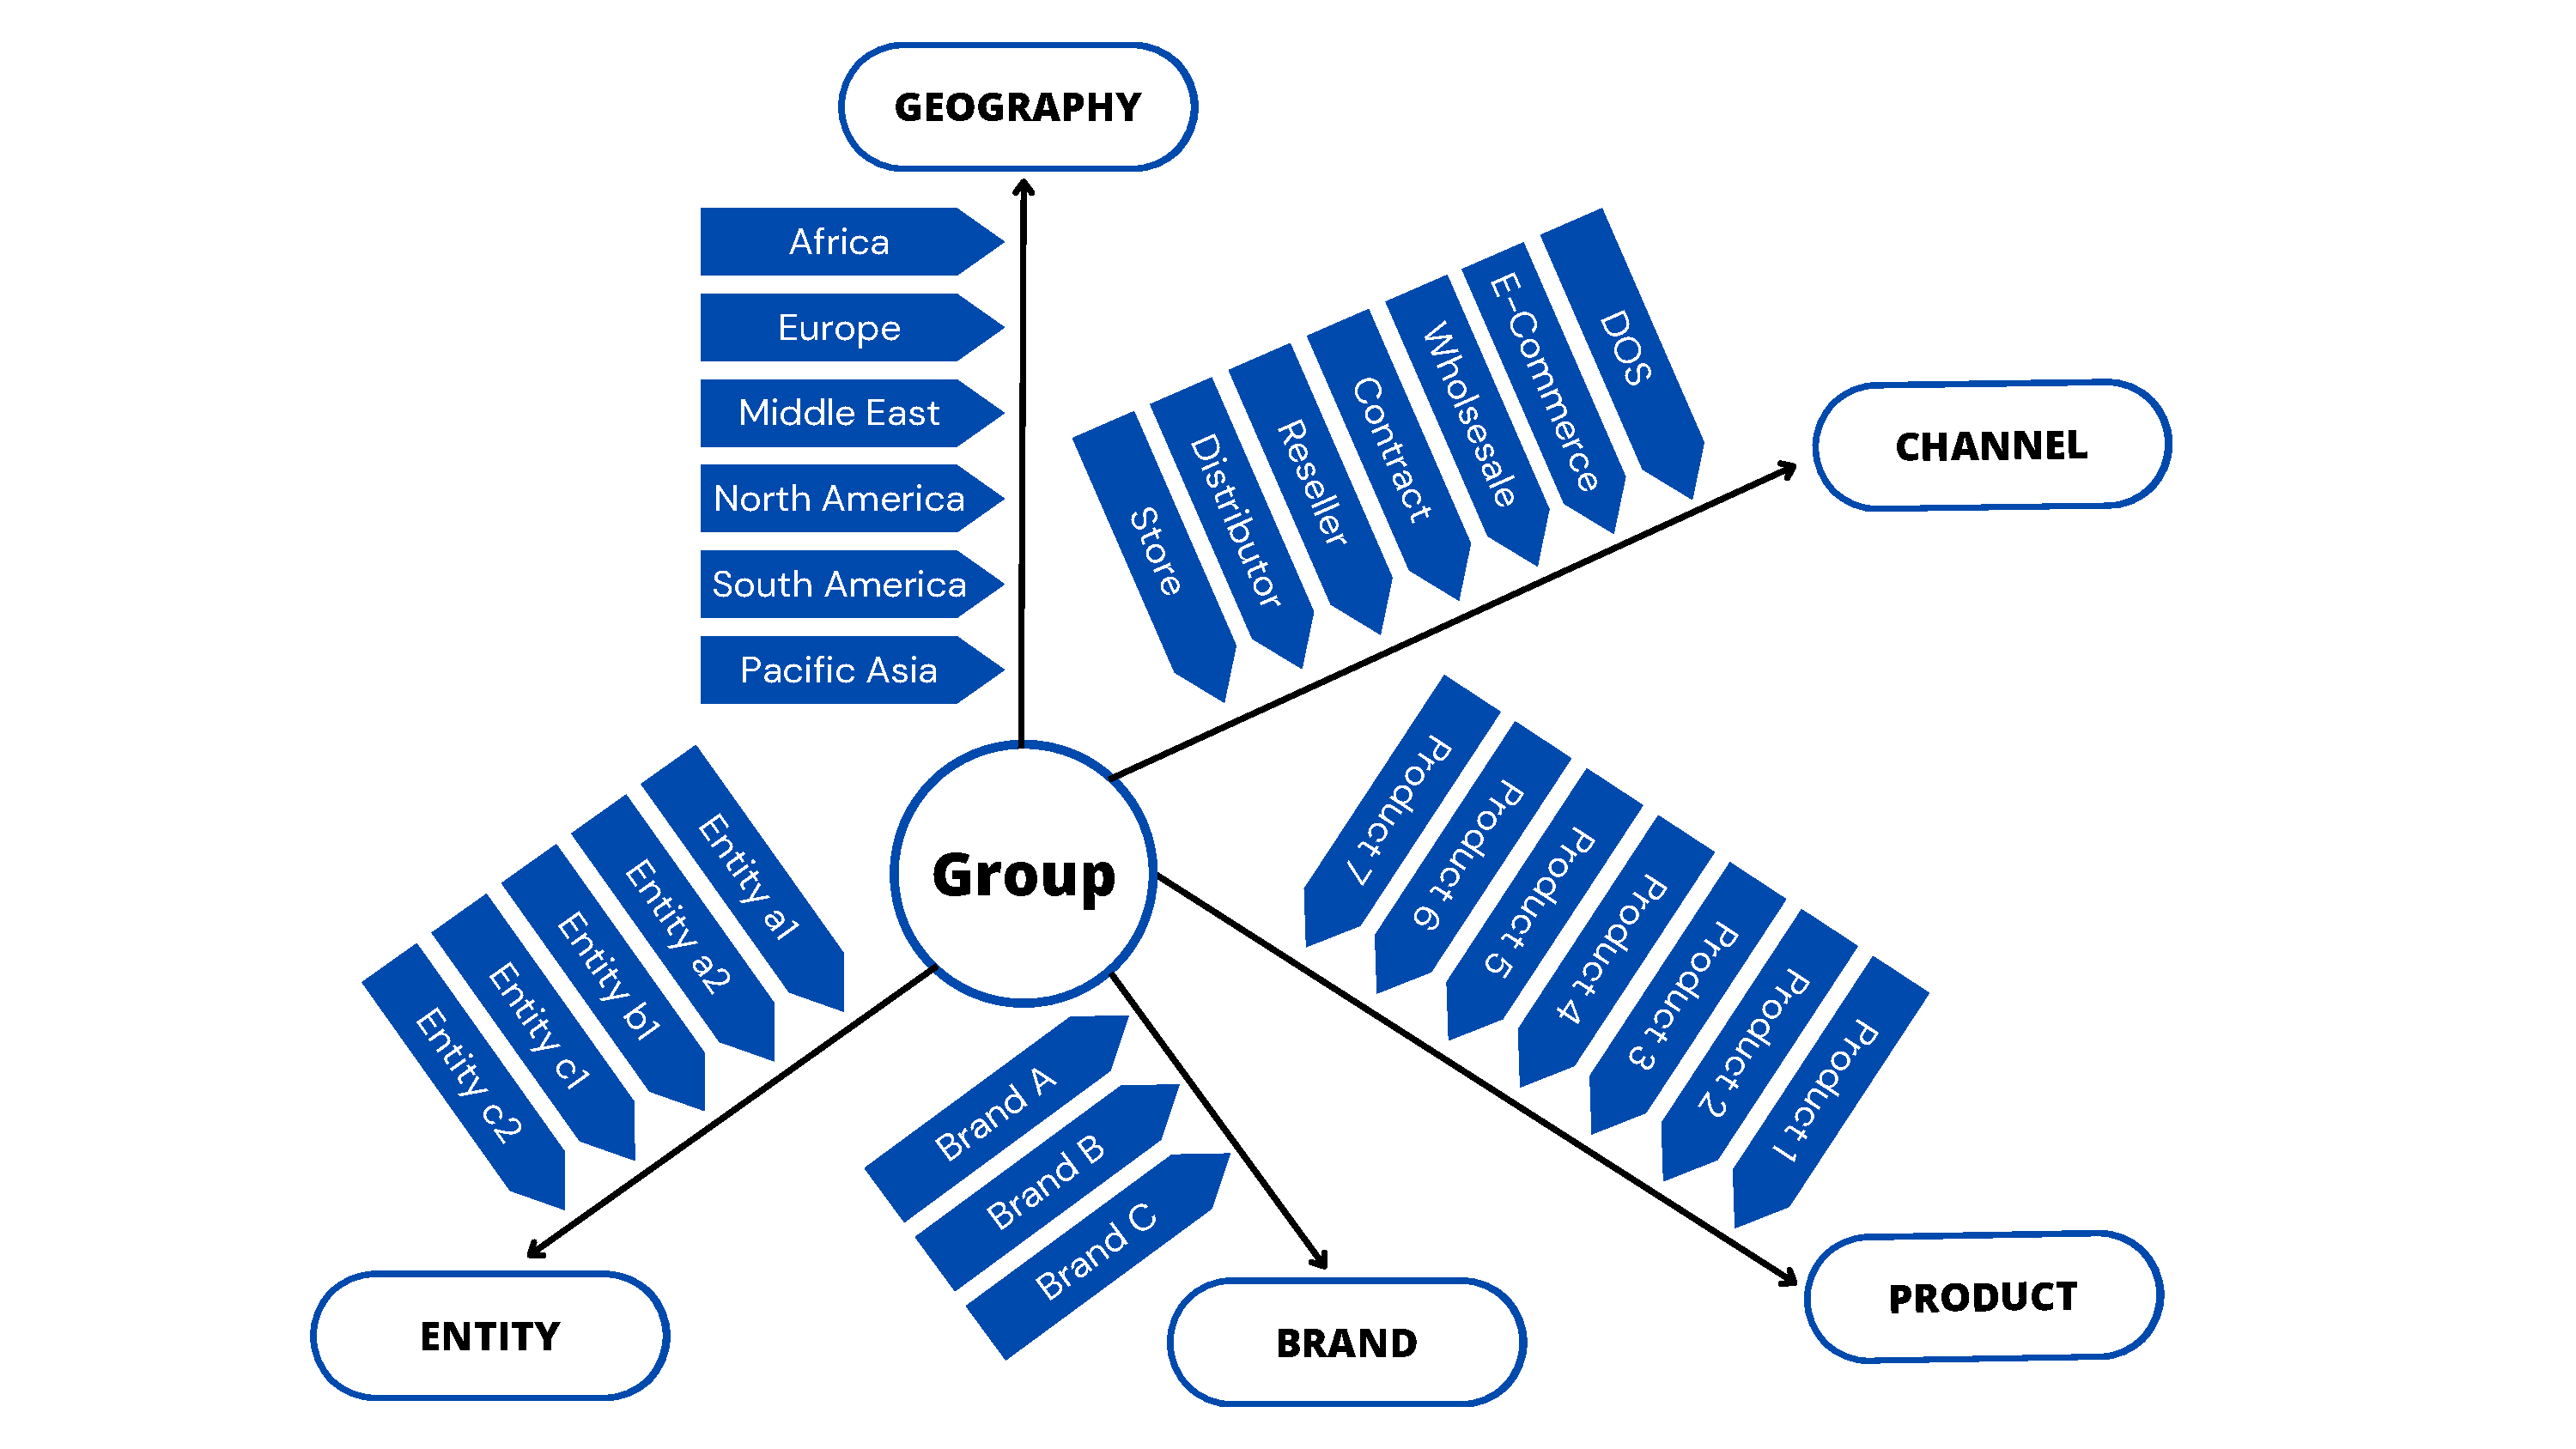
\includegraphics[width=\linewidth]{figures/dimensions.pdf}
	\caption{Dimensions of Analysis}
	\label{fig:dimensions}
\end{figure}

As we can see in figure \ref{fig:dimensions}, the activities of the Holding Group will be evaluated under five different dimensions of analysis: geography, channel, product, brand and Entity.
%
The geography dimension helps analyze financial and operational data based on different geographic regions, thus enabling the Holding Group to understand the performance of its entities across different countries, states, or regions. 
%
The first step to implement such dimension is to determine the levels of geography that are relevant for the analysis, such as country, state, city, or region.
%
Here, the geography dimension include three main geographical groups - EMEA (Europe, Middle East, Africa), Americas and APAC (Asia-Pacific) - which are further subdivided in smaller areas like Middle East, Nordics, Greater China and others.
%
The product dimension allows for a detailed analysis of revenue, costs, and profitability across various product lines, enabling users to analyze data and get insights based on different products.
%
The brand dimension enables analysis and reporting based on different brands owned or managed by the Holding Group. It helps assess brand performance, market share, and customer preferences.
%
The Entity dimension allows for analysis and reporting based on individual entities within the Holding Group, allowing the assessment of the performance of each Entity separately and in comparison within each others.
%
Finally, the channel dimension allows for analysis based on different distribution channels used by the companies to deliver the products and helps assess sales performance and customer preferences across the various channels. 

Once dimensions have been defined, the next crucial step is to load and map the data within the EPM solution and, specifically, to the Financial Consolidation and Close Solution (FCCS). 
%
To populate the dimensions with data, the Holding Group needs to collect financial data from all the Entities as illustrated in figure \ref{fig:dataload}.
%
Of course, different Entities have different data collection tools and methodologies, ranging from ERP software solutions, Excel spreadsheets, BI tools or cloud solutions.
%
Each Brand is responsible for collecting the financial data of the entities that belong to it, which will be transformed and adapted in order to meet the standards for loading.  
%
FCCS allows users to integrate financial data from various sources, such as ERP systems, spreadsheets, and other data sources by means of pre-built connectors that allow users to easily integrate data.

Connectors are software components that enable different applications or systems to communicate and exchange data with each other. 
%
They act as intermediaries, allowing data to flow between two different systems that may use different data formats or data protocols.
%
In FCCS, connectors provide a standardized interface for connecting different systems for integrating data, allowing them to communicate using a specific data format and protocol.

\begin{figure}[ht]
	\centering
	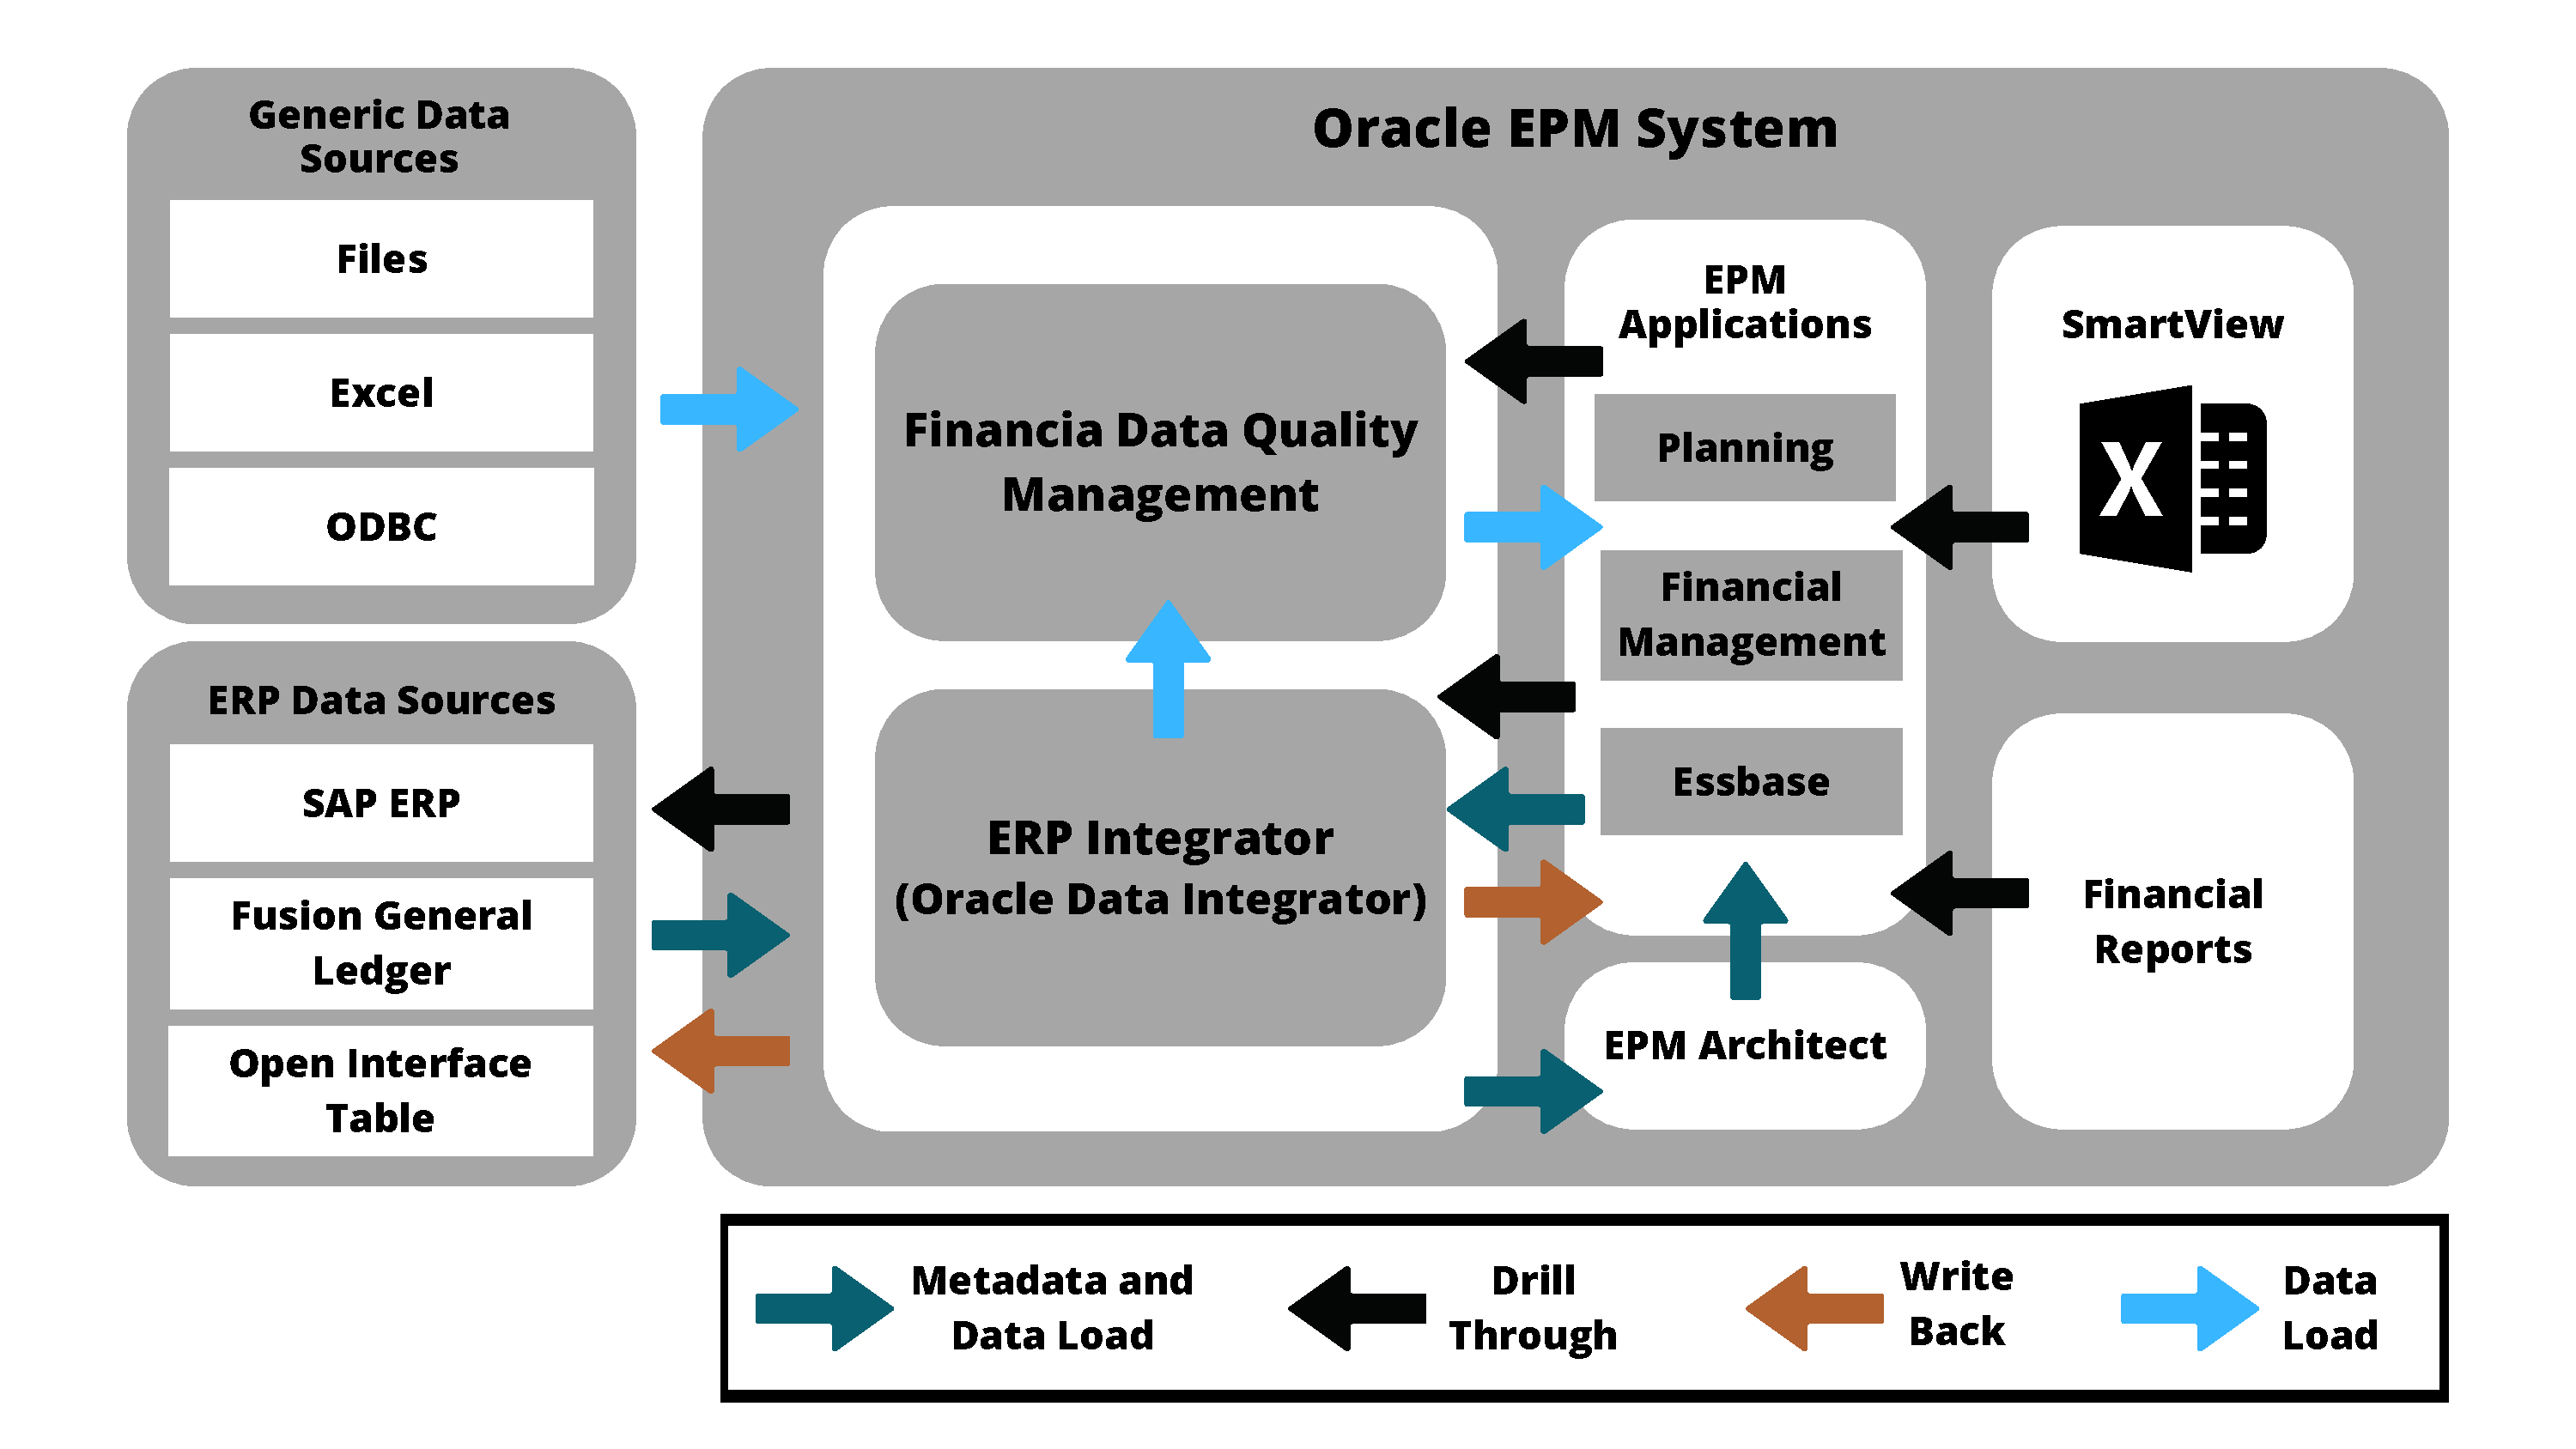
\includegraphics[width=\linewidth]{figures/data-load.pdf}
	\caption{Data Collection Process Across the EPM System}
    \floatfoot{Source: Oracle User's Guide} 
	\label{fig:dataload}
\end{figure}

At the same time, FCCS allows users to map data from different sources to the appropriate dimensions and members, thus ensuring that data is correctly integrated and consolidated even if it comes from different systems with different structures.
%
Data mapping refers to the process of aligning data from different source systems to the dimensions and members in a target system.
%
It involves identifying the relevant data elements in the source system, and then mapping them to the appropriate dimensions and members in the target system. 
%
This process requires an understanding of the data structures and formats used in the source and target systems, as well as the business logic and rules governing the mapping process.
%
Effective data mapping is critical for ensuring the accuracy and completeness of data integration and migration processes; if data is not mapped correctly, it may be lost, duplicated, or incorrectly integrated, resulting in errors and inconsistencies in the target system. 

\begin{figure}[htbp]
	\centering
	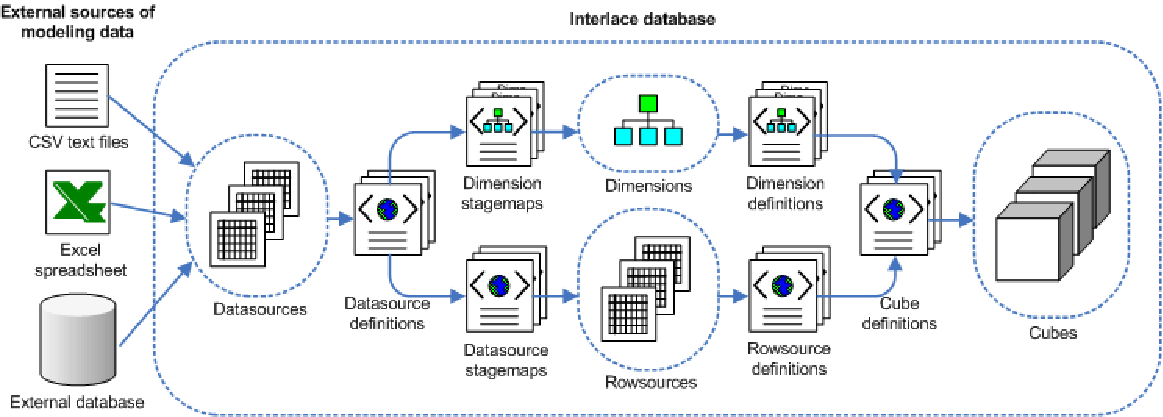
\includegraphics[width=\linewidth]{figures/data-mapping.pdf}
	\caption{Mapping and Modeling Data from Diverse Sources}
    \floatfoot{Source: Oracle User's Guide}
	\label{fig:mapping}
\end{figure}

Figure \ref{fig:mapping} illustrates the relationship and the flow of data among various modeling elements:
%
as we can see, users can model data either creating a model using the data designer integrated in the system or importing a model using XML meatadata definition files.
%
The data coming from different sources is loaded into data-sources, which are relational tables in the integrated planning database where copies of external modeling data are stored. 
%
According to the data-source definitions, the columns to use are set, while stage maps map data-sources to row sources or dimensions in the planning database. 
%
One data-source can be mapped to more than one row source.
%
When data-sources are mapped to dimensions, the system maps the names from the tabular data-source to the elements of the dimension’s hierarchical structure. 
%
In addition to mapping columns to dimension members at all levels, the system maps the attributes of the dimension members and specifies the relationship (for example, parent-child).
%
The mapping among cubes allows data values in one cube to flow to data values in another cube. 
%
Since the cubes have different structures, the mapping defines how the data should flow; the mapping is like a table join in a relational database: it defines the common dimensions and how to map or join them.

To identify how source dimensionality translates to target dimensionality, member mappings based on source values are used. 
%
Member mappings are referenced during the data load, enabling the Data Management to determine how to dimensionalize the data that is loaded to the target application. 
%
They define relationships between source members and target dimension members within a single dimension. 
%
This is done by creating a member mapping for each target dimension which, based on the business logic, can have different levels of granularity:

\begin{enumerate}
    \item Explicit: the source value is matched exactly and replaced with the target value. For example, source value ``ABC'' is replaced with target value ``123''.
    \item Between: the range of source values is replaced with a single target value. For example, a range from ``001'' to ``010'' is replaced as one value: ``999''. 
    \item In: it enables a list of non-sequential source values to be mapped to one target value. For example, you could have source accounts 1503, 1510, and 1515 map to the target account 15000010.
    \item Multi-Dimension: it enables users to define member mapping based on multiple source column values. For example, if the source value combination is Entity-001,002 Department-ABC, XYZ Account-1222, 1333, then the target value assigned for Account Dimension is 1200.
    \item Like: the string in the source value is matched and replaced with the target value.  For example, the source value ``Department'' is replaced with the target value ``Cost CenterA''.
\end{enumerate}

When processing the source values for transformations, multiple mappings may apply to a specific source value. 
%
The order of precedence is Explicit, Between, In, Multi-Dimension, and Like. 
%
Once data have been mapped into the correct dimensions and members, the next step is to transform them to match the requirements of FCCS. 
%
Data transformation is a critical aspect of data integration and management as it enables organizations to convert data from various source systems into a consistent format that can be used for financial consolidation and reporting.
%
This process involves applying various rules and calculations to ensure that data is accurate, complete and consistent.
%
More in details, some specific data transformation techniques used in FCCS include:

\begin{enumerate}
    \item Data Validation: Checking data for errors, inconsistencies, and missing values, and correcting or flagging issues as necessary.
    \item Data Aggregation:  Combining data at various levels of granularity to produce summary values for reporting and analysis.
    \item Data Translation: Converting data from one language or currency to another to facilitate consolidation and reporting.
    \item Intercompany Elimination: Adjusting data to eliminate transactions between related entities or companies, in order to produce accurate consolidated financial statements.
\end{enumerate}

FCCS provides a range of tools and features to support data transformation, including pre-built mapping templates, data validation rules, and built-in calculations and consolidation methods. 
%
At the same time, this application provides a range of features to help users manage data governance.
%
This aspect is particularly important for a Holding Group as it helps ensuring that data is managed and protected consistently across all entities, while guaranteeing that data usage is compliant with regulations and best practices.
%
Effective data governance ensures that data is managed and protected, while being compliant with regulations such as GDPR, the Italian Data Protection Law, and CCPA \footnote{The GDPR (General Data Protection Regulation) applies to any company that processes the personal data of individuals located in the European Union, regardless of where the company is located. The Holding Group must also comply with the Italian Data Protection Law, which regulates the processing of personal data in Italy, as well as other data protection regulations in the countries where its brands are located, including U.S with the CCPA (California Consumer Privacy Act).}, reducing the risk of penalties, fines, or legal actions.
%
At the same time, it ensures that sensitive data is protected from unauthorized access,  reducing the risk of data breaches and consequential reputational damage.
%
On a more technical level, data governance ensures that data is shared in a controlled and secure manner, while ensuring that data is managed and used consistently across all entities, improving standardization and efficiency.

The process of data load runs continuously to keep the EPM system up-to-date with respect to the financial situation of the Holding Group in real-time.
%
It is therefore important to update the process systematically to meet changes in business operations and allow the system to run smoothly, providing an accurate representation of reality.
%
Oracle FCCS serves as a powerful tool within the EPM framework as it empowers organizations to streamline financial consolidation, close processes, and reporting. 

The process of consolidating financial data from multiple entities, business units and subsidiaries is automated, ensuring accurate and consistent consolidation by applying predefined rules, intercompany eliminations, currency translations, and other necessary adjustments.
%
At the same time, FCCS facilitates the entire close management process\footnote{The close management process refers to a series of activities undertaken by businesses to finalize their financial records for a specific period, typically at month-end, quarter-end, or year-end. It involves tasks such as reconciliations, adjusting entries, financial reporting, review and approval, and documentation.} by providing a centralized system to track, manage, and review the progress of close tasks. 
%
It allows organizations to define close calendars, assign responsibilities, and monitor the completion of close activities.
%
The integration capabilities of FCCS enable a smooth flow of data to other Oracle EPM solutions, such as Oracle Planning for planning, reporting and forecasting purposes - as shown in figure \ref{fig:planning-fccs}.
%
By seamlessly loading data from FCCS to the planning system, the Holding Group can leverage the consolidated financial data for budgeting, forecasting, and scenario planning. 
%
This native integration ensures a cohesive and holistic approach to financial management, facilitating data-driven decision-making across the organizations.
%
Data from FCCS are copied periodically into Planning with specific rules set to keep data aligned between the two environments.
%
The import rule is automatic but it can also be launched at Group level. 

\begin{figure}[htbp]
	\centering
	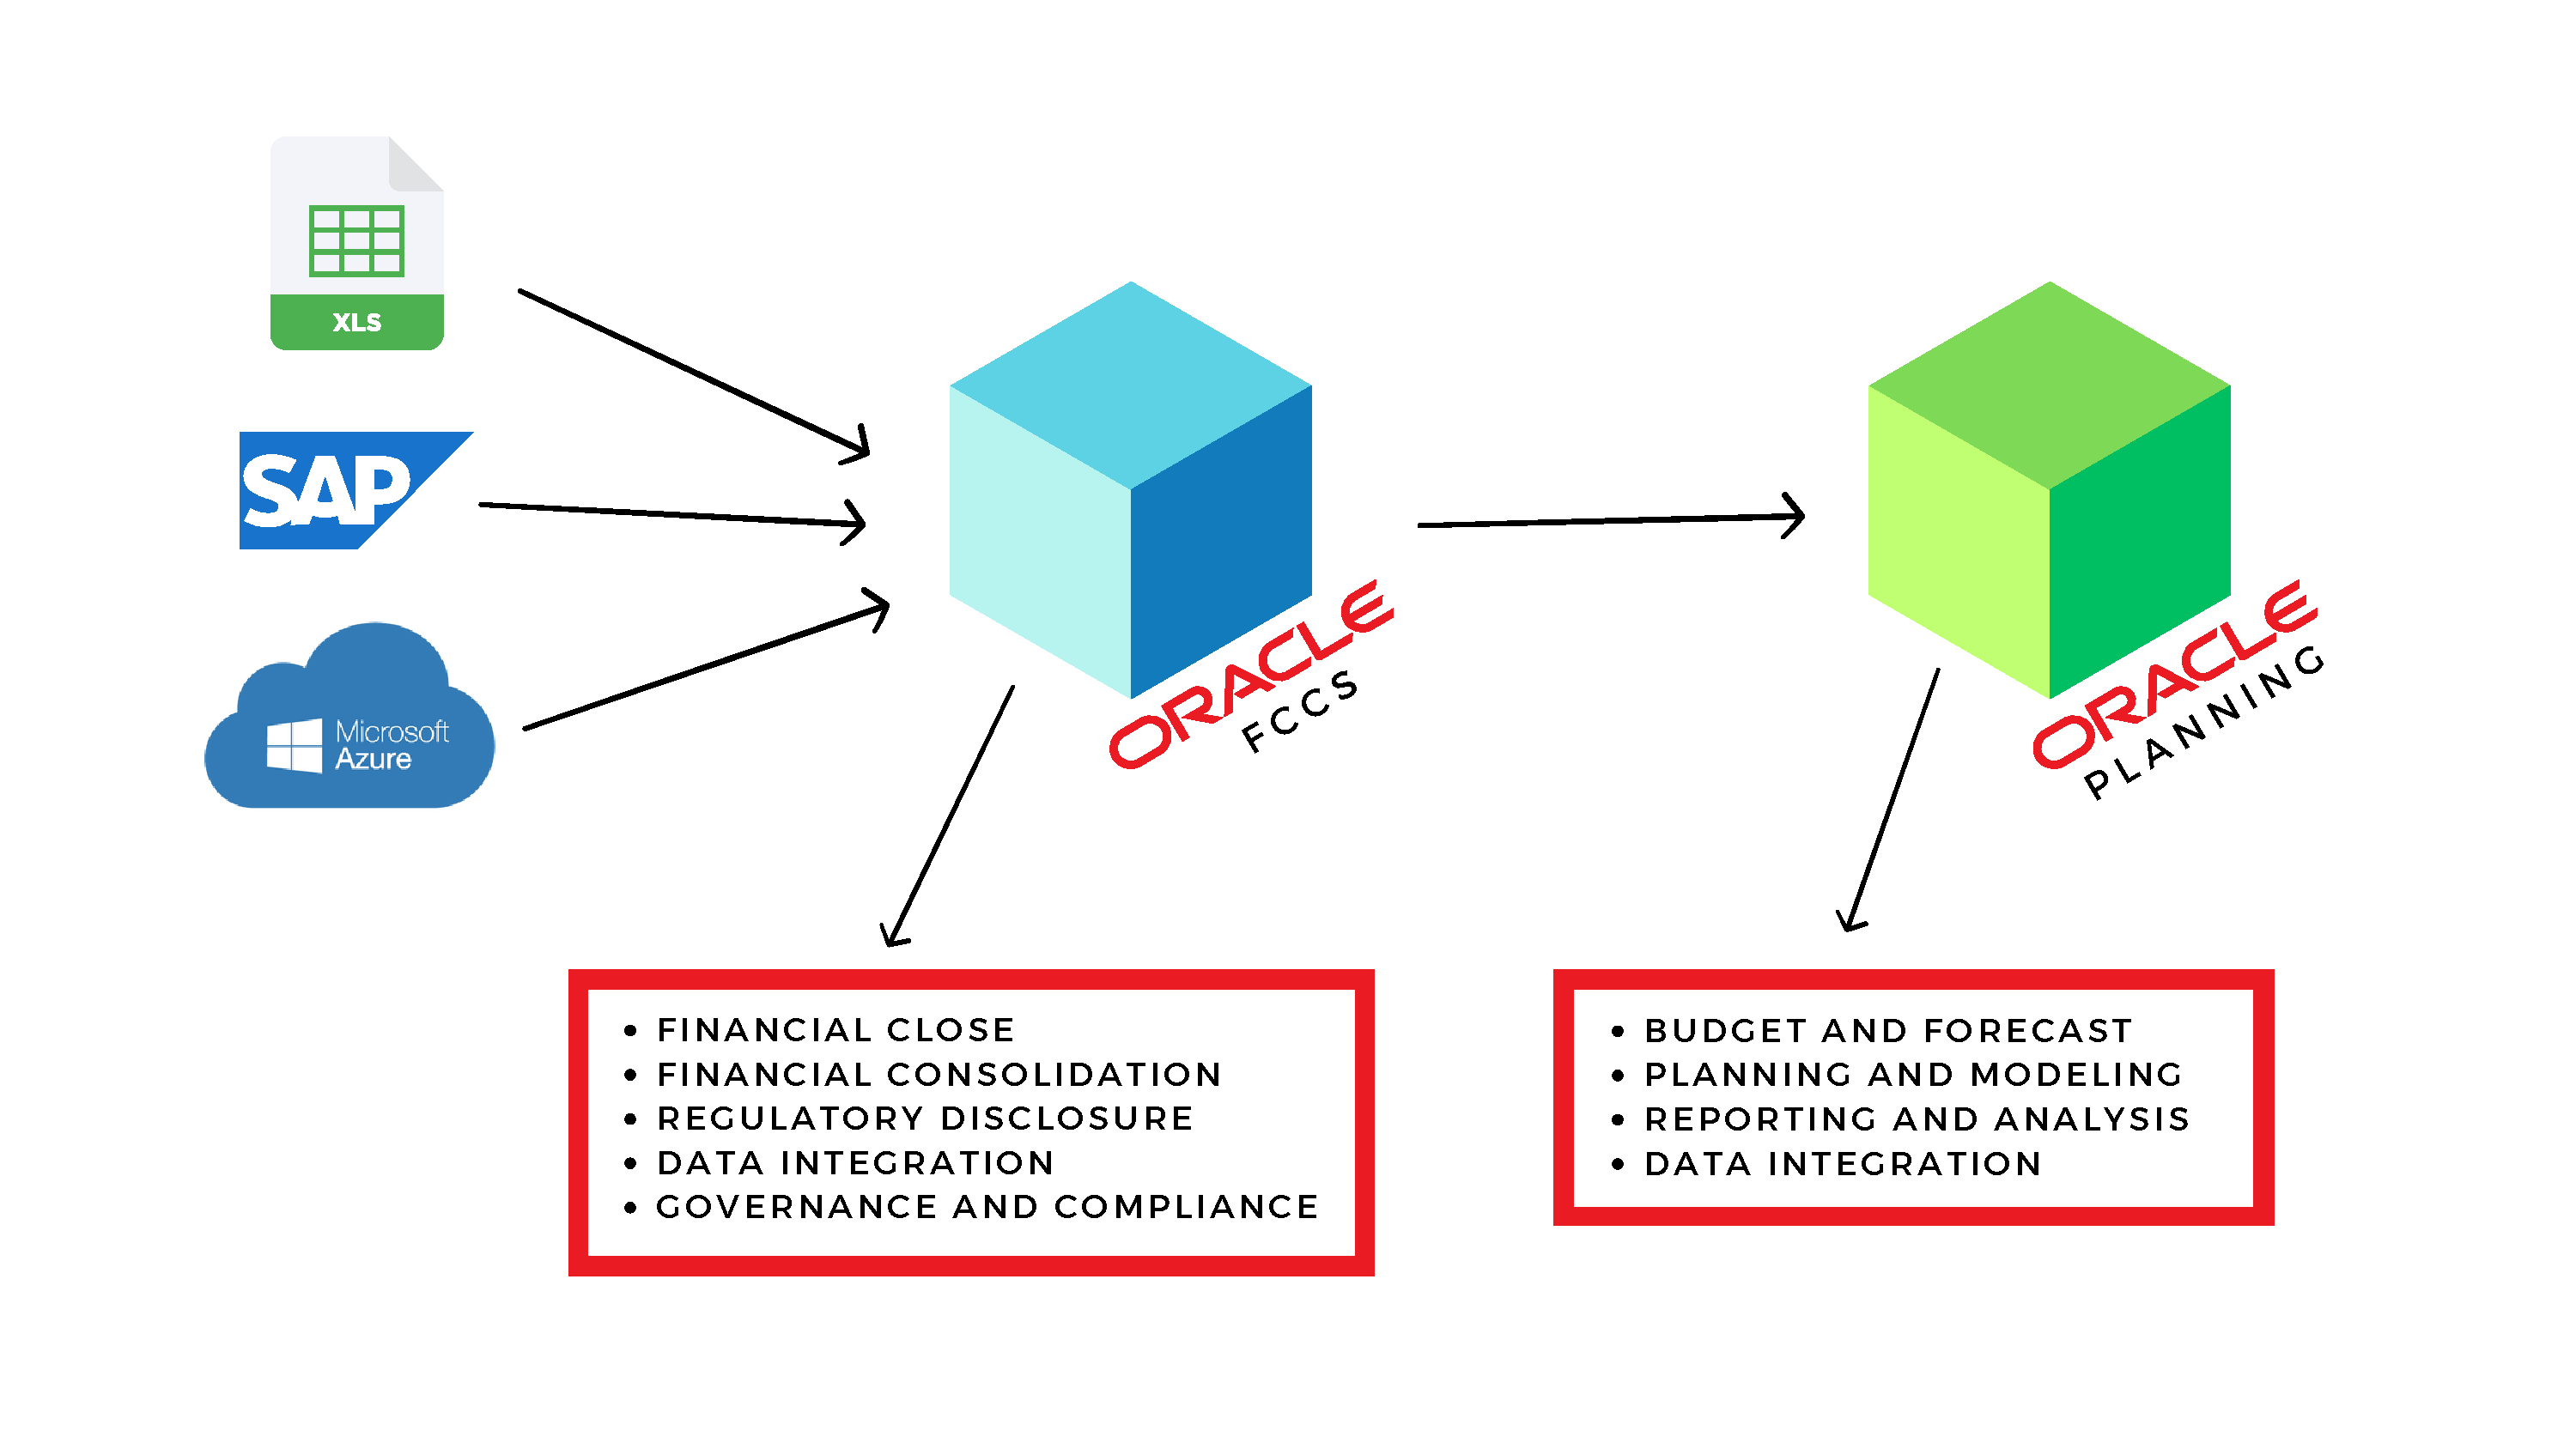
\includegraphics[width=\linewidth]{figures/planning-fccs.pdf}
	\caption{Integration between FCCS and Oracle Planning}
	\label{fig:planning-fccs}
\end{figure}

The integration between Oracle FCCS and Oracle Planning allows organizations to seamlessly transfer financial data from the consolidated financial system to the planning system. 
%
This automated data flow eliminates the need for manual data entry and reduces the risk of errors that can occur during manual data transfer.
%
By leveraging the data from Oracle FCCS, organizations can align their planning and budgeting processes with the actual financial results, as the system incorporates the most up-to-date and accurate financial information from the consolidation process.
%
The automatic data loading from FCCS to Oracle Planning ensures data integrity and consistency throughout the planning and budgeting cycle; any changes or updates made in the consolidated financial system are automatically reflected in the planning system, enabling users to work with real-time data for their budgeting and forecasting activities.
%
Furthermore, the automation of data loading from to Oracle Planning enhances the efficiency of the planning and budgeting process by reducing the time and effort required for data reconciliation and ensuring that the planning system is always synchronized with the latest financial information. 

Oracle Planning offers a robust set of functionalities that empower businesses to streamline their financial processes and make informed decisions. 
%
With activities like planning and modeling, budgeting and forecasting together with reporting and analysis, Oracle Planning provides a comprehensive suite of tools and features to support organizations in their journey towards optimized financial performance. 
%
 Let's explore the key functionalities of Oracle Planning in detail.

\paragraph{Planning and Modeling:} 

Planning and modeling refers to the process of creating strategic plans, setting goals, and developing models that simulate various business scenarios.
%
By modeling different scenarios, organizations can assess the potential impact of changes and make informed decisions based on those insights.
%
Oracle Planning allows users to create multiple planning scenarios to assess the impact of different business variables on financial outcomes, enabling organizations to evaluate various what-if scenarios and make informed decisions based on different assumptions.
%
Users can model and forecast financial results based on key business drivers such as sales volume, pricing or production capacity.
%
This approach helps organizations understand the relationships between drivers and financial outcomes.
%
Oracle Planning also includes specialized features for workforce planning and modeling which enable organizations to forecast and manage their human resources-related expenses, such as salaries, benefits, and workforce allocation, ensuring alignment between workforce planning and overall financial planning.

\paragraph{Budgeting and Forecasting:}

Budgeting and forecasting involve the creation of financial plans and projections for a specific period.
%
Budgeting focuses on allocating financial resources to different areas of the organization, while forecasting predicts future financial performance based on historical data and anticipated changes. 
%
Oracle Planning provides a user-friendly interface for creating and managing budgets: users can input, review, and adjust budget data, leveraging predefined templates and workflows to streamline the budgeting process. 
%
At the same time, organizations can perform rolling forecasts using Oracle Planning, allowing them to update and revise their forecasts periodically based on actual performance and changing business conditions. 
%
This helps to keep forecasts accurate and relevant throughout the planning period.

\paragraph{Reporting and Analysis:}

Reporting and analysis encompass the generation of financial statements, performance reports, and key performance indicators (KPIs) to assess the financial health and performance of an organization. 
%
Reporting and analysis facilitate data-driven decision-making, provide visibility into financial performance, and support effective communication with stakeholders.
%
Oracle Planning enables the generation of financial statements, including balance sheets, income statements, and cash flow statements: users can create customized reports that provide insights into financial performance, variances, and key metrics. 
%
The solution supports various reporting formats, including tabular reports, graphical dashboards, and interactive visualizations.
%
The system also empowers users to perform ad-hoc analysis by providing intuitive tools and interfaces. 
%
Users can explore data, drill down into details, create personalized views, and conduct multidimensional analysis to uncover trends, patterns, and outliers.
%
With Oracle Planning, organizations can analyze and compare actual performance against budgeted or forecasted figures in order to identify areas of variance and take corrective actions as necessary.
%
Finally, Oracle Planning offers interactive dashboards with real-time data visualizations and KPI monitoring that users can use to create personalized dashboards to track performance, monitor progress, and gain insights into key business metrics.

\section{Data transformations and calculations}

In Oracle Cloud EPM, data transformation and calculation are fundamental aspects that enable organizations to derive meaningful insights from data. 
%
Within the EPM environment, these capabilities are achieved through the utilization of business rules.
%
This section delves into the world of data transformation and calculation in Oracle Cloud EPM, focusing on how business rules drive these processes.
%
Data transformation and calculation in Oracle Cloud EPM play a key role in aggregating, consolidating, and manipulating data across the multidimensional cubes of the EPM application.
%
Business rules serve as the mechanism to define and automate complex calculations, allowing organizations to streamline their financial modeling, scenario planning, and other analytical operations.
%
Within this section, we will explore the specific programming language used for creating business rules, known as Calculation Manager Script\footnote{The Calculation Manager script can be considered a programming language tailored specifically for performing calculations and data transformations in the context of EPM applications. Although it has its own syntax and structure, it shares similarities with other programming languages, such as control flow structures, variables, functions, and operators.}. 
%
This proprietary language provides a robust set of functions, operators, and syntax elements tailored to the EPM environment, empowering users to construct intricate calculations with precision and flexibility.
%
Additionally, this section elucidates the mechanics of how business rules operate across the multidimensional cubes. 
%
It explores the sequence and flow of calculations, the retrieval of data from source locations, and the storage of results in target locations, ensuring consistency and accuracy throughout the EPM application.

In Oracle Cloud EPM, data transformation and calculation capabilities are achieved through the use of business rules. 
%
Business rules provide a powerful mechanism for defining and automating complex calculations, data transformations, and validation logic within the multidimensional cubes of the EPM application.
%
They are composed of several key components that work together to define and automate calculations and data transformations. 

\paragraph{Members:}
Members are the individual elements or dimensions within a multidimensional data set. 
%
They represent specific elements, such as products, countries, time periods, or accounts. 
%
In the context of business rules, members are used to identify the source and target data elements involved in calculations, defining the scope of calculations and determining which data points are affected by the rule.

\paragraph{Formulas:}
Formulas define the calculation logic within a business rule.
%
They specify how the source data members are combined and transformed to derive the desired results.
%
Formulas can include mathematical operations, aggregation functions, conditional statements, and references to other members or variables. 
%
They determine how data is manipulated, consolidated, allocated, or transformed during the calculation process.

\paragraph{Conditions:}
Conditions are logical expressions that determine whether a particular calculation or action should be performed. 
%
They evaluate specific criteria based on member values or other conditions and determine the flow of execution within the business rule. 
%
Conditions can be used to include or exclude certain data points, define branching logic, or control the application of specific calculations based on specific conditions being met.

\paragraph{Variables:}
Variables are used to store and manipulate intermediate results or temporary values within a business rule. %
They can be declared and assigned values dynamically during rule execution. 
%
Variables enhance the flexibility and efficiency of calculations by allowing users to store and reuse values, perform calculations using intermediate results, and simplify complex logic by breaking it down into smaller, manageable steps.

\paragraph{Templates:}
Templates are predefined structures or patterns that can be used as a starting point for creating business rules. 
%
They provide a framework that includes placeholders for members, formulas, conditions, and other components. 
%
Templates offer a consistent and standardized approach to developing business rules, saving time and effort by providing a starting point and ensuring adherence to best practices.

\paragraph{Member Range:}
Member range specifies a subset of members within a dimension that should be considered during the calculation process. 
%
It allows users to define specific criteria for selecting members dynamically based on their properties or attributes. 
%
Member ranges can be used to restrict the calculation scope to a subset of data, improve performance by reducing unnecessary calculations, or target specific members for allocation or consolidation purposes.

\paragraph{Metadata Loop:}
The metadata loop is a powerful feature in Oracle Cloud EPM that allows for dynamic calculation and manipulation of members and their properties. 
%
It enables iterating over members of a dimension and performing calculations or actions based on their metadata values. 
%
The metadata loop provides flexibility in handling members with changing properties, such as applying specific calculations only to members that meet certain criteria or dynamically adjusting formulas based on metadata values. \\

Business rules operate across the multidimensional cubes of the EPM application by applying calculations to specific intersections of dimensions. 
%
The rules are executed during the data consolidation and aggregation processes, allowing for real-time calculations and updates to the cube data.
%
When a business rule is triggered, it retrieves data from the specified source locations, performs the defined calculations using the specified logic and formulas, and then stores the results in the target locations within the multidimensional cube. 
%
This process ensures consistent and accurate calculations across the entire EPM application.

When writing a business rule, it is important to follow a systematic approach to ensure accurate and efficient calculations.
%
The first step is to understand the dimensions and the data flow across the cube.
%
The goal is to gain a deep understanding of how the dimensions are structured in the EPM application, identifying the key dimensions involved in the calculation process and understand how data moves across the cube.
%
This understanding is crucial to accurately define the source and target members in the business rule.
%
Then, it is important to determine the purpose of the rule by clearly defining the objective of the business rule and understanding the specific calculation or data transformation to achieve.
%
At the same time, the scope of the rule should be defined.
%
The scope of the rule regards the subset of members - source members and target members - to be considered in the calculation process. 

\begin{figure}[htbp]
	\centering
	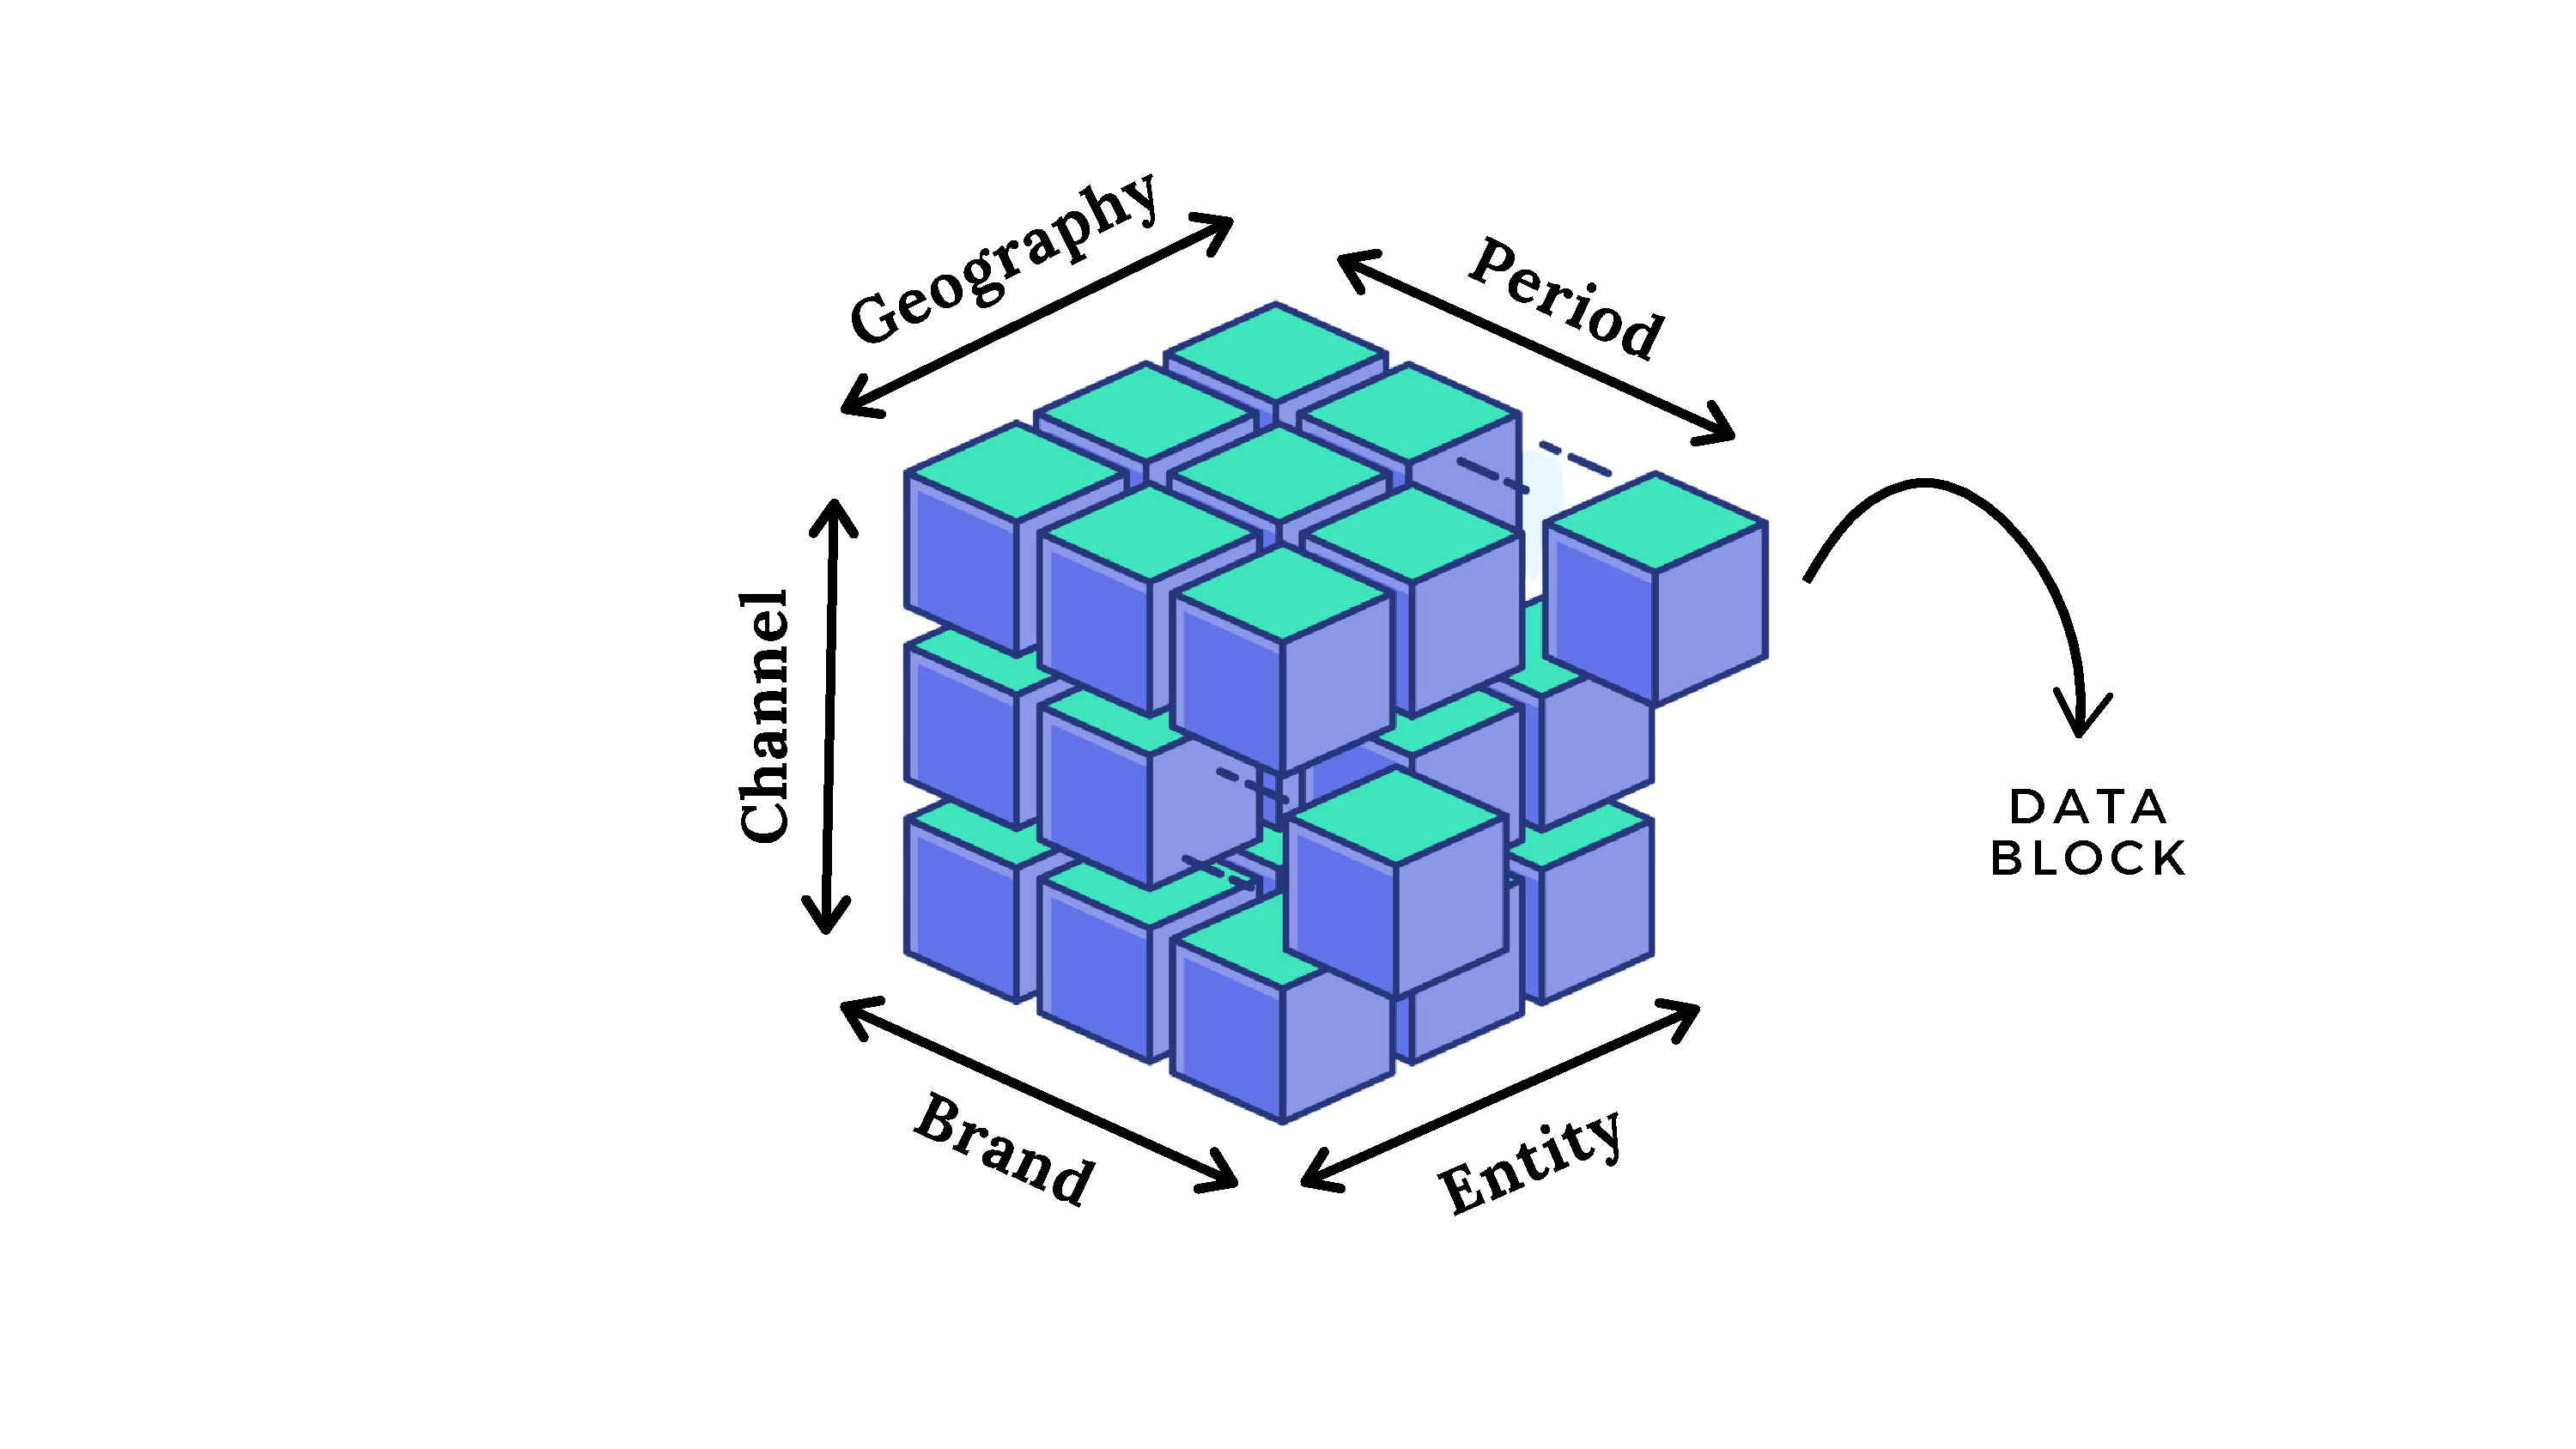
\includegraphics[width=\linewidth]{figures/cube.pdf}
	\caption{Data Block in a Multidimensional Database}
	\label{fig:cube}
\end{figure}

Before making calculations, it is necessary to create blocks in the cube which allow for efficient data management and calculation process.
%
Blocks provide a structured and organized format for storing data in a multidimensional cube: by partitioning the cube into blocks, data can be stored and retrieved more efficiently. 
%
Each block contains a subset of the cube's data, typically defined by specific combinations of dimension members, allowing for faster access to data during calculations and queries, as only relevant blocks need to be accessed.
%
At the same time, creating blocks helps optimize the performance of data processing operations as, by dividing the cube into manageable chunks, calculations can be performed more efficiently. 
%
During calculations, only the blocks affected by the specific calculation or data transformation need to be processed, reducing the overall processing time. 
%
This partitioning also facilitates parallel processing, allowing multiple blocks to be processed simultaneously, further improving performance.
%
Partitioning the cube into blocks provides flexibility in managing data because blocks can be selectively loaded or unloaded based on data requirements, thus optimizing storage space. 
%
This flexibility also extends to data backups and recovery processes, as individual blocks can be easily backed up, restored, or migrated independently, enabling efficient data management and maintenance.

Once the scope has been defined, the calculations to perform should be set.
%
In this step we will use the Calculation Manager script or graphical interface to define the calculations, formulas, and logic required for the business rule. 
%
By all means, the calculation logic should be written using the appropriate syntax, functions, operators, and control structures.
%
Once that we are sure that the calculations align with the purpose and scope of the rule, we can test and validate the business rule to ensure its correctness and accuracy. 
%
To do so, we can use the validation tools provided by Oracle Cloud EPM to identify any syntax errors, formula inconsistencies or logical issues. 
%
At the same time, it is essential to review the calculations and logic to ensure they align with the intended purpose and produce the expected results.
%
Once the rule is validated, we can deploy it to the appropriate EPM application, ensuring that the rule is assigned to the relevant data intersections and is ready for execution. 
%
At this point, we can set up any necessary schedule or trigger for the rule execution, considering factors such as frequency, dependencies, and performance requirements.
%
Now, we can use Smart View, the Microsoft Office Excel add-in, to access and analyze the results of the business rule.
%
To do so, we need to connect Smart View to the EPM application and retrieve the data that has been calculated or transformed by the rule, verifying that the results align with the expected outcomes and meet the defined requirements.

%----------------------------------------------------------------------------------------
\chapter{Business Rules for Efficient Planning}
\label{chap:cmyactivity}
%----------------------------------------------------------------------------------------

During the internship, I actively participated in diverse aspects of this EPM project, gaining hands-on experience in configuring, customizing, and optimizing the EPM solution. 
%
This chapter delves into my contributions and experiences during the internship period, specifically focusing on two essential implementations within the Enterprise Performance Management project: cost allocation and intercompany management. 
%
While working on various sections of the EPM solution, these two implementations emerged as particularly relevant, showcasing how Oracle Cloud EPM can meet specific needs of customers.
%
The chapter begins by providing an overview of the importance of cost allocation and intercompany management in the context of Enterprise Performance Management. 
%
Then, it highlights the challenges and complexities associated with these areas and delves into my practical journey in addressing them during the implementation process.
%
Furthermore, it offers insights into the strategies, methodologies, and tools employed to establish efficient cost allocation processes and streamline intercompany transactions, while discussing the challenges encountered during the implementation.
%
In conclusion, this chapter delves into best practices and lessons learned throughout the implementation process, reflecting on the key takeaways, including the importance of data accuracy, stakeholder engagement, clear communication, and continuous improvement. 

\section{Cost allocation}

% Describe Cost Allocation
Cost allocation is a financial management process that involves assigning and distributing costs to various departments, divisions, products, or projects within an organization. 
%
Within the Holding Group, cost allocation plays a crucial role in accurately determining the financial performance and profitability of each Entity.
%
It helps in evaluating the contribution of each Entity and each Brand to the overall success of the Holding Group, enabling effective decision-making regarding resource allocation, investment opportunities, and strategic planning.
%
Cost allocation policies can be personalized to align with the specific needs and characteristics of the company. 
%
These policies take into account various factors such as the nature of business operations, the structure of the Holding Group, the legal relationship between entities and the strategic objectives of the parent company.

To define such policies, the Holding Group undertook the following steps:

\begin{enumerate}
    \item Identifying cost drivers: cost drivers are the factors that directly influence the recording of costs. Here, the Holding Group identified three variables as driver, which are Brand, Geography and Channel of Distribution.
    \item Allocating direct costs: direct costs, which can be easily attributed to specific departments, are allocated based on a straightforward allocation basis.
    \item Allocating indirect costs: indirect costs, which cannot be directly attributed to specific areas, require more complex allocation methods. These methods involve the use of allocation drivers that reflect the usage or benefit received by different departments.
    \item Determining granularity level: the granularity level refers to the degree of detail at which costs are allocated within the Holding Group. 
\end{enumerate}

% What the customer want
The Holding Group aims at establishing an automated system that can accurately allocate costs based on predefined rules, taking into account the validity of drivers with respect to the starting intersections to allocate.
%
By implementing this system, the Holding Group seeks to achieve greater efficiency, accuracy, and transparency in their cost allocation practices.
%
At the same time,  by establishing clear rules and leveraging the platform's capabilities, they aim to streamline their financial processes, improve decision-making, and gain better insights into the performance and profitability of the entities within the Holding Group.

The Holding Group has identified three key dimensions for cost allocation: Brand, Geography, and Channel. 
%
For each dimension, they have categorized the starting intersections into three types: 

\begin{enumerate}
    \item ``Specific Member'': the variable is given, meaning that the expense was incurred by a specific Brand (for Brand), in a specific country (for Geography) and through a specific channel of distribution (for Channel).
    \item ``No Member'': the variable is not given and the expense should be allocated in order to identify the attributable Brand, Geography or Channel.
    \item ``Member to Allocate'': the variable is given, but it represents a lower level of detail. The expense was incurred in a broad geographical area (like EMEA or APAC), regards a group of entities under the same sub-group or belong to a class of channels of distribution without identifying the specific one. In this case, the expense should be allocated with a greater level of detail.
\end{enumerate}

This results in a total of 27 possible combinations of starting intersections to allocate across the dimensions.
%
By all means, a starting intersection in which Brand, Geography and Channel are all specific, already has the maximum level of detail and there is no need to allocate the expense, leading to 26 possible combinations to considerate.

\begin{figure}[htbp]
	\centering
	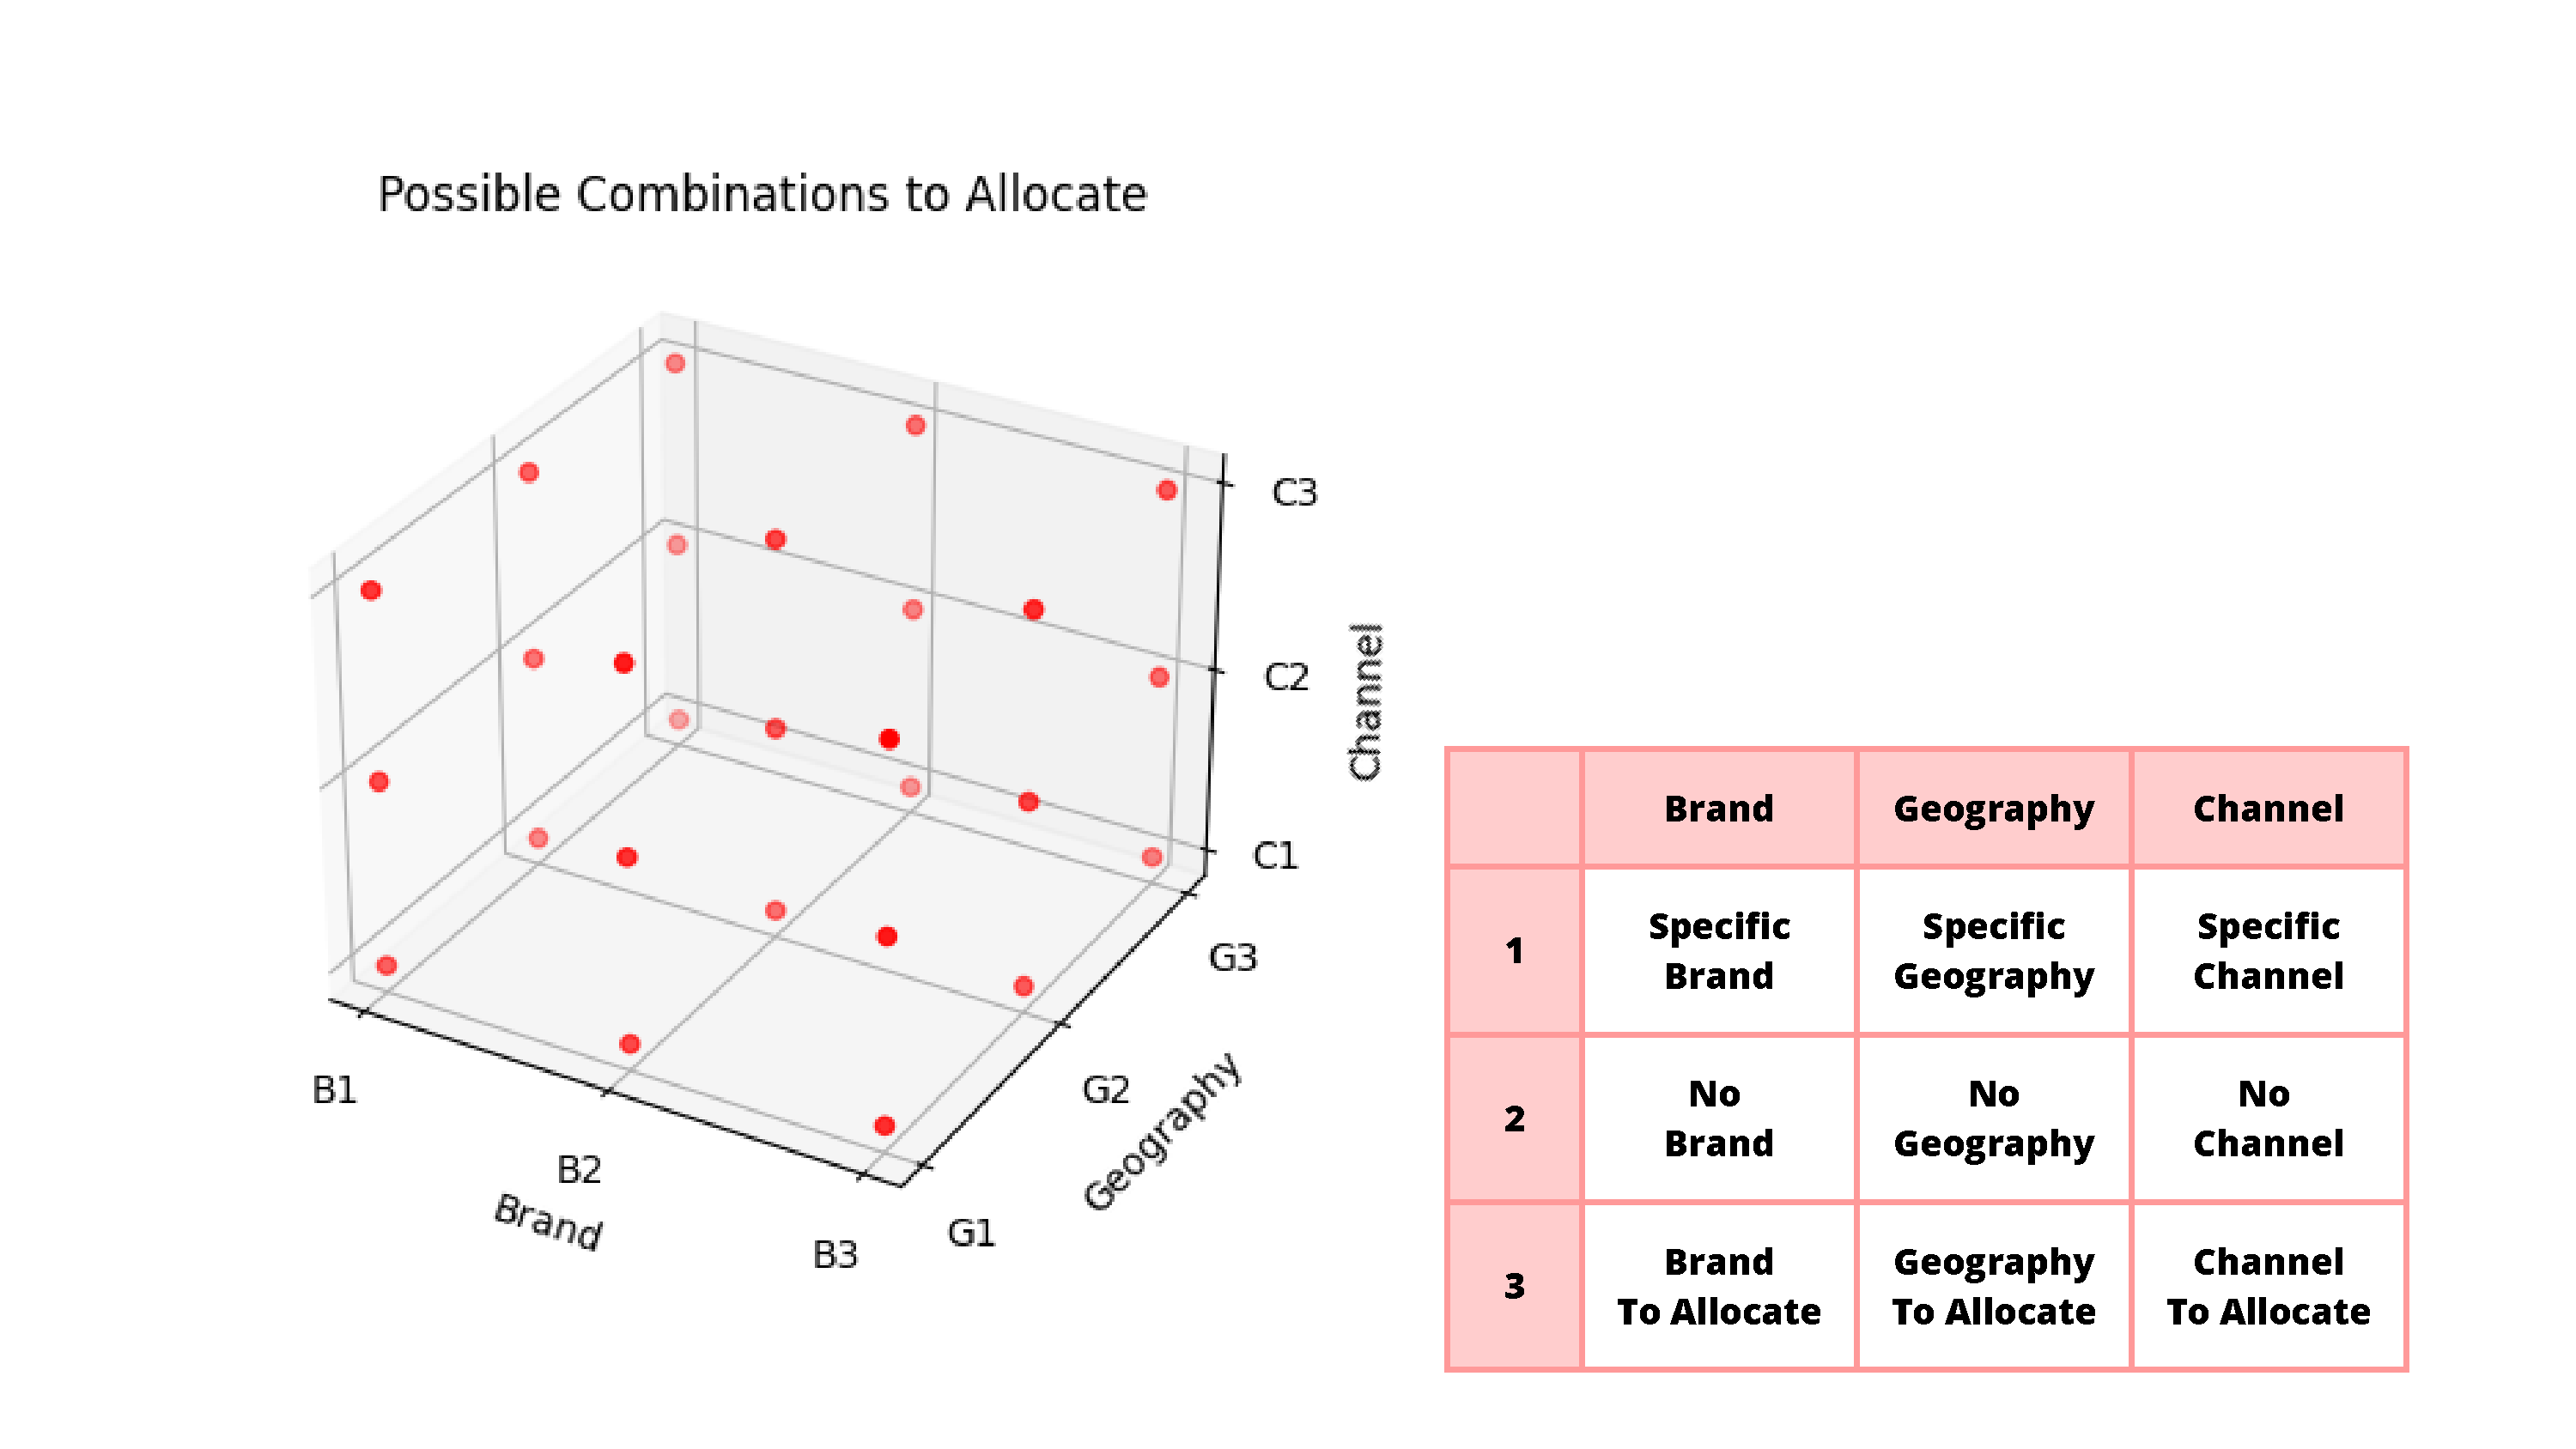
\includegraphics[width=\linewidth]{figures/combinations.pdf}
	\caption{Combinations of Brand-Geography-Channel to Allocate}
	\label{fig:combos}
\end{figure}

Figure \ref{fig:combos} displays all the possible combinations to which the costs to allocate may belong; for example, we may have sales, general and administrative expenses (SG\&A) incurred by a specific brand (B1), in a specific geographical area without the detail of the country (G3), through an unknown channel of distribution (C2).

One of the significant challenges faced during the cost allocation process is the lack of detailed information in the intersections of the variables Brand, Geography, and Channel.
%
This limitation arises from the fact that different Entities employ different tools for collecting financial data and, at the same time, each Entity follows its own business policy, resulting in variations in the granularity levels at which data is collected.
%
In the context of cost allocation, it refers to the extent to which expenses are tracked and categorized based on various dimensions and explains the presence of different types of intersections to allocate based on the different detail level.
%
For example, one Entity may have a more granular approach, capturing expenses at a detailed level for each specific Brand, Geography and Channel combination. 
%
On the other hand, another Entity might adopt a more aggregated approach, grouping expenses at a higher level and lacking the necessary level of detail in these intersections.
%
The lack of consistent granularity levels across the Holding Group poses challenges when it comes to allocate costs.
%
It becomes difficult to accurately allocate expenses when there are discrepancies in the level of detail captured for the variables considered, which hampers the ability to precisely attribute costs to specific intersections.
%
To address this challenge, the implementation project recognizes the need to establish standardized guidelines and policies for allocating expenses based on specific drivers whose validity is based on the intersection to allocate.

In this regard, the Holding Group has defined three different types of drivers for each dimension:

\begin{enumerate}
    \item ``Specific Driver'': the driver allocates the cost on a specific member for the dimension Brand, Geography or Channel.
    \item ``All Driver'': the driver allocates the cost on the same member of the starting intersection.
    \item ``Multiple Driver'': the driver allocates the cost on a combination of specific members for the dimension Brand, Geography or Channel.
\end{enumerate}

These drivers play a critical role in determining the allocation of costs within the identified intersections.
To meet the customer's requirements, the implementation project aims to develop an automated system that can handle the complex task of cost allocation. 
%
The system will incorporate specific rules that govern the validity of drivers based on the starting intersections; this ensures that costs are allocated accurately and in accordance with the predefined allocation methodology.

\begin{figure}[htbp]
	\centering
	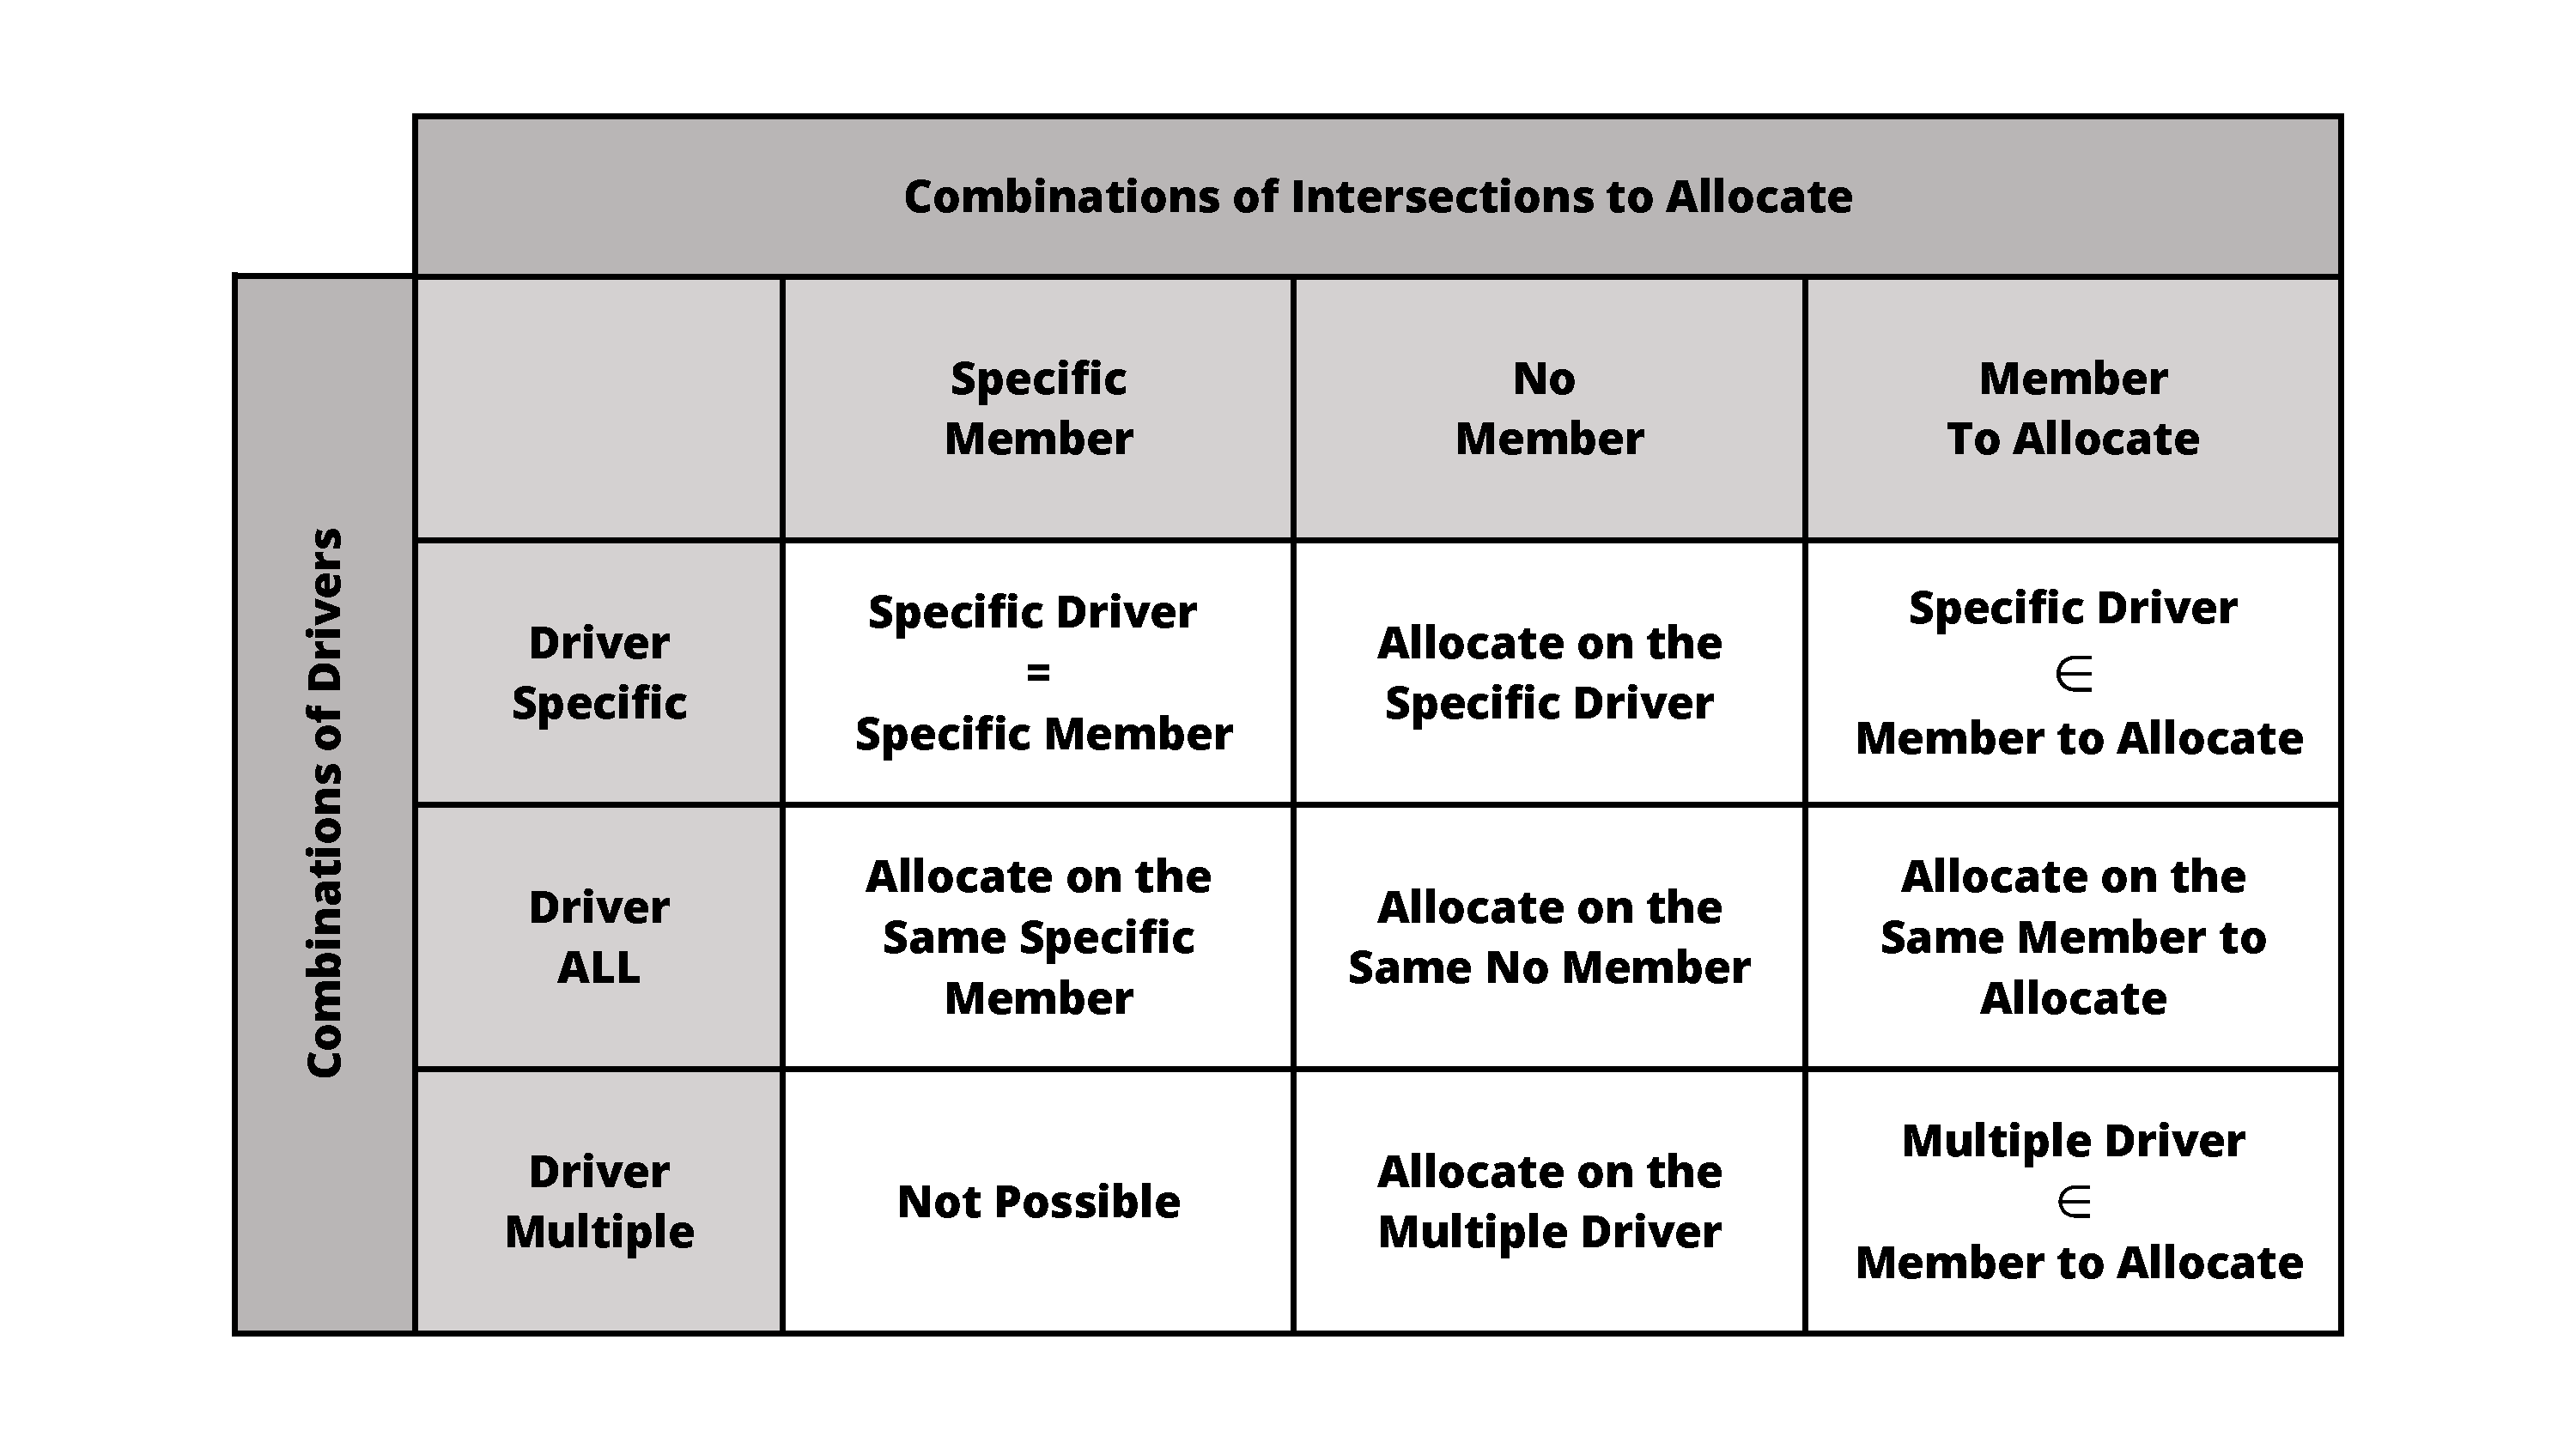
\includegraphics[width=\linewidth]{figures/driver-table.pdf}
	\caption{Allocation Rules based on Driver Validity}
	\label{fig:driver}
\end{figure}

Figure \ref{fig:driver} illustrates the validity of the drivers based on the combinations of Brand, Geography and Channel for the intersections to allocate.
%
As we can see, the different drivers allocate costs in different destinations based on the nature of the  starting intersection:
%
A specific driver is valid with a specific member only if they are equivalent; we cannot move a cost from a specific Brand, Geography or Channel to another one.
%
On the contrary, when the detail for a dimension is not given (No Member), the cost can be allocated on any specific member or combination of specific members.
%
With Members to allocate, where the detail of the dimension is of high level, the specific driver is valid only if the member on which the cost should be allocated belong to the same group of the Member to Allocate.
%
For example, a cost with EMEA as member of the Geography dimension, can be allocated only on countries which belong to the EMEA geographical grouping (Europe, Middle East and Africa).
%
The same guiding principle goes for multiple driver, meaning that a Member to Allocate can be allocated on multiple specific members as long as they belong to the same group for that dimension.
%
Ultimately, ``Driver ALL''is always valid and allocates the cost on the same member of the starting intersection for the dimension in which it is used.

As a general rule, the cost for a specific intersection of Brand, Geography and Channel can be allocated only if the driver covers the intersection entirely.
%
For instance, figure \ref{fig:allocation} exhibits two examples of allocations: as we can see, both cases starts from a cost to allocate that has a specific Brand (Brand A), EMEA and E-commerce as a starting intersection for the dimensions Brand, Geography and Channel, which amounts to € 1,000.00.
%
The drivers for both the cases are composed of a specific Brand, a multiple driver for Geography and a ``Driver All'' for the Channel dimension.
%
Specifically for the first case, 70\% of the cost should be allocated on the intersection ``Brand A, Spain, E-commerce'' and the remaining 30\% on the intersection ``Brand A, China, E-commerce'', while in the second case, 70\% of the cost belongs to ``Brand A, Spain, E-commerce'' and 30\% goes to ``Brand A, Germany, E-commerce''.
%
Nevertheless, the first case represents an invalid driver and only the driver of the second case can correclty allocate the cost.
%
The first driver does not cover the intersection entirely as 30\% of the driver is invalid, due to the fact that China does not belong to EMEA but is part of the APAC group.
%
The second driver, on the other hand, accurately allocate the cost entirely as it meets all the rules that govern the validity of the drivers.

\begin{figure}[ht]
	\centering
	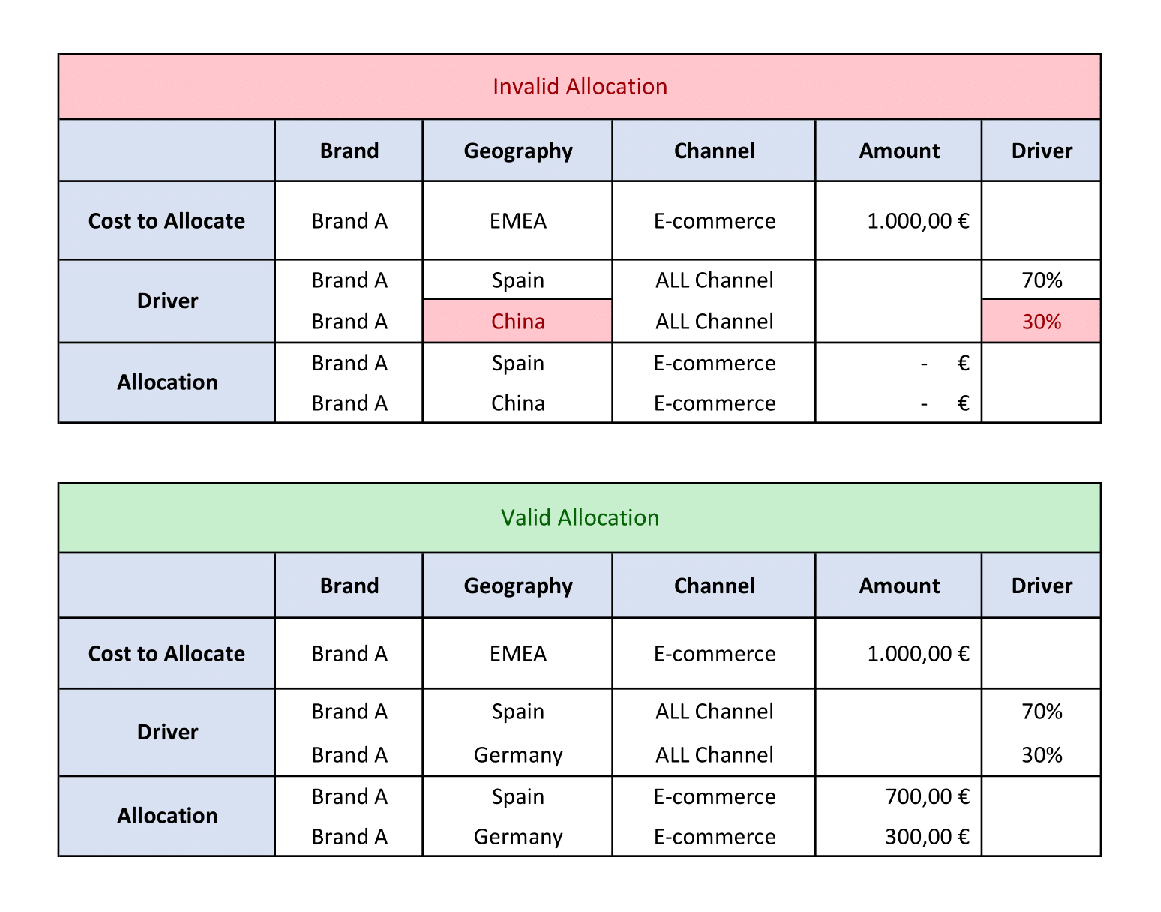
\includegraphics[width=\linewidth]{figures/allocation.pdf}
	\caption{Valid and Invalid Allocation Example}
	\label{fig:allocation}
\end{figure}

The first step for the implementation process of the allocation system involved the gathering of the requirements from the client in order to understand deeply the business processes, financial goals and the allocation needs.
%
Once the allocation logics have been defined, the next step is to design the solution.
%
This involves identifying all the possible combinations of drivers and intersections to allocate, as well as defining the technical elements needed for the implementation.
%
In particular, the key elements needed for the allocation system, include:

\begin{enumerate}
    \item Business Rules: the allocation process was split into two phases, each of which was carried out through a specific business rule.
    \item Members: several new members were added to the relevant dimensions, including Brand, Geography, Channel and some technical dimensions which allow the correct functioning of the rule.
    \item User Defined Attributes (UDA): to identify the members to allocate, a new UDA was added to the specific members.
    \item Forms: an ad hoc input form was designed to allow users to input the drivers for the allocation.
    \item Reports: some reports were created in order to check the outcome of the allocation process.
\end{enumerate}

\begin{figure}[htbp]
	\centering
	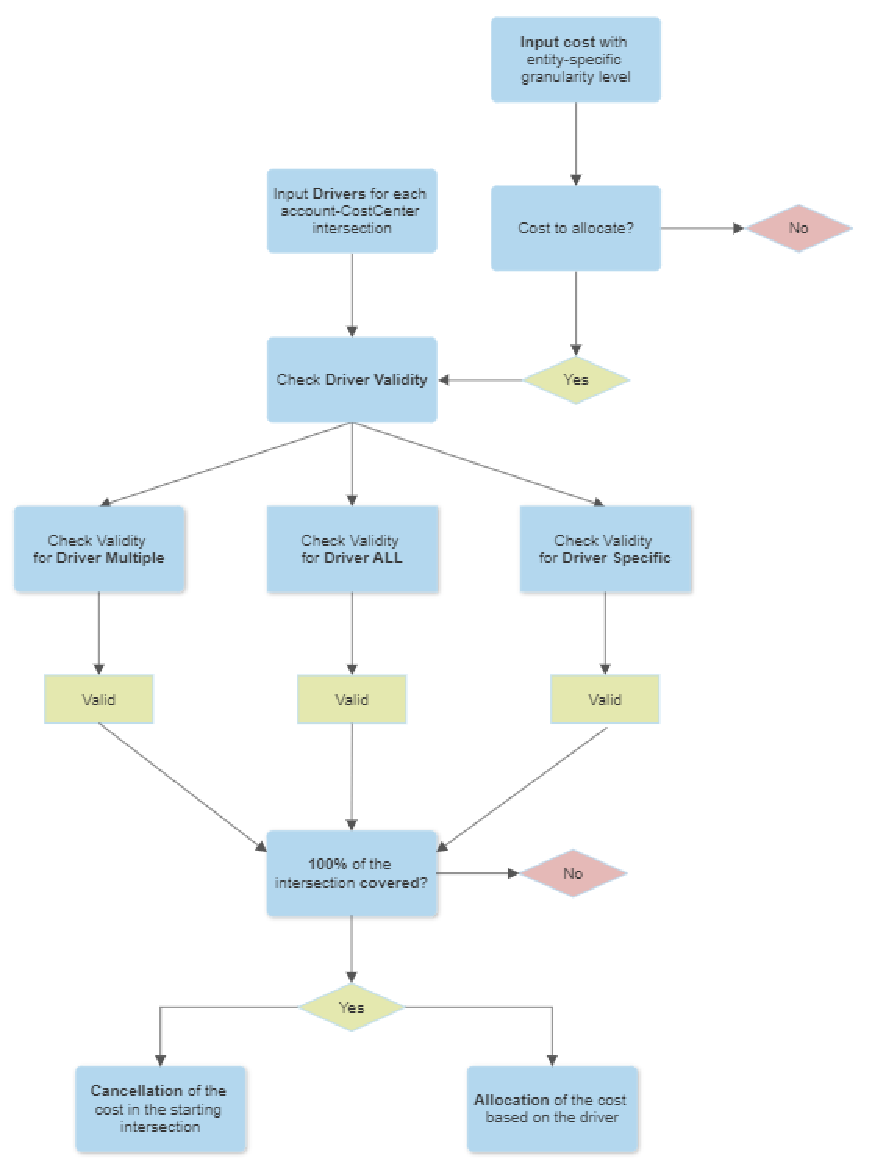
\includegraphics[width=\linewidth]{figures/process.pdf}
	\caption{Steps Involved in the Allocation Process}
	\label{fig:process}
\end{figure}

To effectively manage the allocation system, the process was broken down into two tasks carried out by two respective business rule: the first rule deals with the driver while the second one performs the allocation of the cost.
%
Drivers are defined by the Holding Group each month and are designed in order to cover all the combinations of accounts and cost centers (one driver for each intersection).
%
The first rule is purely technical and functional to the second one: it analyzes the composition of the driver and assigns some flags on predefined support intersections which will be used by the second rule to complete the allocation process.
%
These numerical flags simply categorize each dimension of the driver according to whether the driver is specific, all or multiple.
%
At the same time, it calculates and stores the allocation percentage for each intersection of the driver, which will be multiplied by the amount of the cost to be allocate during the second phase.

Regarding the second rule, figure \ref{fig:process} displays the key logical steps performed by the rule, starting from the retrieval of the value of the driver until the allocation of the cost.
%
The rule starts by checking whether the cost is to allocate, that is when at least one dimension is either ``No Member'' or ``Member to allocate'' and, if this is the case, ti check the driver validity.
%
To do so, it uses the numerical flags applied by the previous rule and compares the driver combination to the combination of Brand, Geography and Channel of the starting intersection to allocate.
%
Once the validity is assessed, the rule proceeds to verify that the driver covers the intersection to allocate entirely.
%
Finally, the rule concludes the process with the cancellation of the cost on the starting intersection, which will be distributed across the dimensions based on the percentages of the driver.
%
As soon as one of the requirements is not met, the rule stops and the cost will remain on the starting intersection.

After implementing the business rules, it is crucial to thoroughly test the allocation system.
%
This involves performing tests with massive launches of data to simulate real-world scenarios, with the purpose of verifying the system's performance, identify any bottlenecks or errors, and ensure that the allocation calculations are accurate and consistent across the various dimensions. 
%
Testing also helps in uncovering any unforeseen issues that may arise during the allocation process.
%
Once the allocation system has been tested and validated, the focus shifts to optimizing its performance. 
%
This was done by identifying and addressing any performance bottlenecks and by fine-tuning the system configuration and calculations to achieve a discrete level of efficiency and responsiveness. 
%
The final step in the implementation process was conducting a User Acceptance Testing (UAT) with the client: during the UAT, the client verified that the allocation system meets the agreed requirements and performs as expected. 
%
During this phase, feedbacks about the functioning of the system are of key importance in order to carry out any necessary adjustments or refinements to the rules.
%
Once the client approves the system, it is ready for release, meaning that the allocation system is deployed in the production environment, enabling users to leverage its capabilities for accurate and efficient allocation of costs across the dimensions of interest.

\section{Intercompany management}

% Describe Intercompany Management
Intercompany transactions refer to financial transactions that occur between entities within the same parent company. 
%
These transactions can involve the transfer of goods, services, or funds between related entities.
%
This concept plays a crucial role within the Holding Group, as it enables the coordination and collaboration between different entities while maintaining centralized control and ownership.
%
By all means, intercompany transactions are a common occurrence, especially for Holding Group with this size and expansion level.
%
These transactions serve various purposes, such as the sharing of resources and services or the transfer of assets across the entities. 
%
However, it is important to note that intercompany transactions can introduce complexities in financial reporting and consolidation: when intercompany transactions are not appropriately accounted for and eliminated during the consolidation process, they can distort the financial statements and create an artificial economic value within the Holding Group.
%
Eliminating intercompany transactions during the consolidation process is crucial for the Holding Group as it helps prevent the duplication of revenues, expenses, assets, and liabilities, which can lead to inflated financial results.
%
At the same time, eliminating intercompany transactions supports the goal of creating a clear and transparent view of the group's operations and finances, allowing stakeholders to evaluate the group's financial performance through reliable financial information.

% What the customer want
To achieve the elimination of intercompany transactions, the Holding Groups requested a specialized system which is able to automate the process of identifying, matching, and eliminating intercompany transactions during the consolidation process.
%
The implementation of such system posed several challenges due to the nature of intercompany transactions and the complexities associated with data protection within the Holding Group.
%
Intercompany transactions involve a two-way relationship between entities: on one side, an Entity records a revenue in its local currency, while on the other side, another Entity incurs a cost. 
%
This creates a complex intersection of financial relationships that need to be accurately identified, matched, and eliminated during the consolidation process.
%
The complexity increases further when considering the concept of data protection: each Entity operates independently and has its own set of financial data, which is confidential and sensitive. 
%
As a result, the different entities cannot have unrestricted access to the financial data of other entities.
%
The challenge arises from the fact that the intercompany elimination process requires access to financial data from multiple entities to accurately identify and eliminate intercompany transactions.
%
However, allowing unrestricted access to financial data poses a significant risk to data privacy and security.

\begin{figure}[htbp]
	\centering
	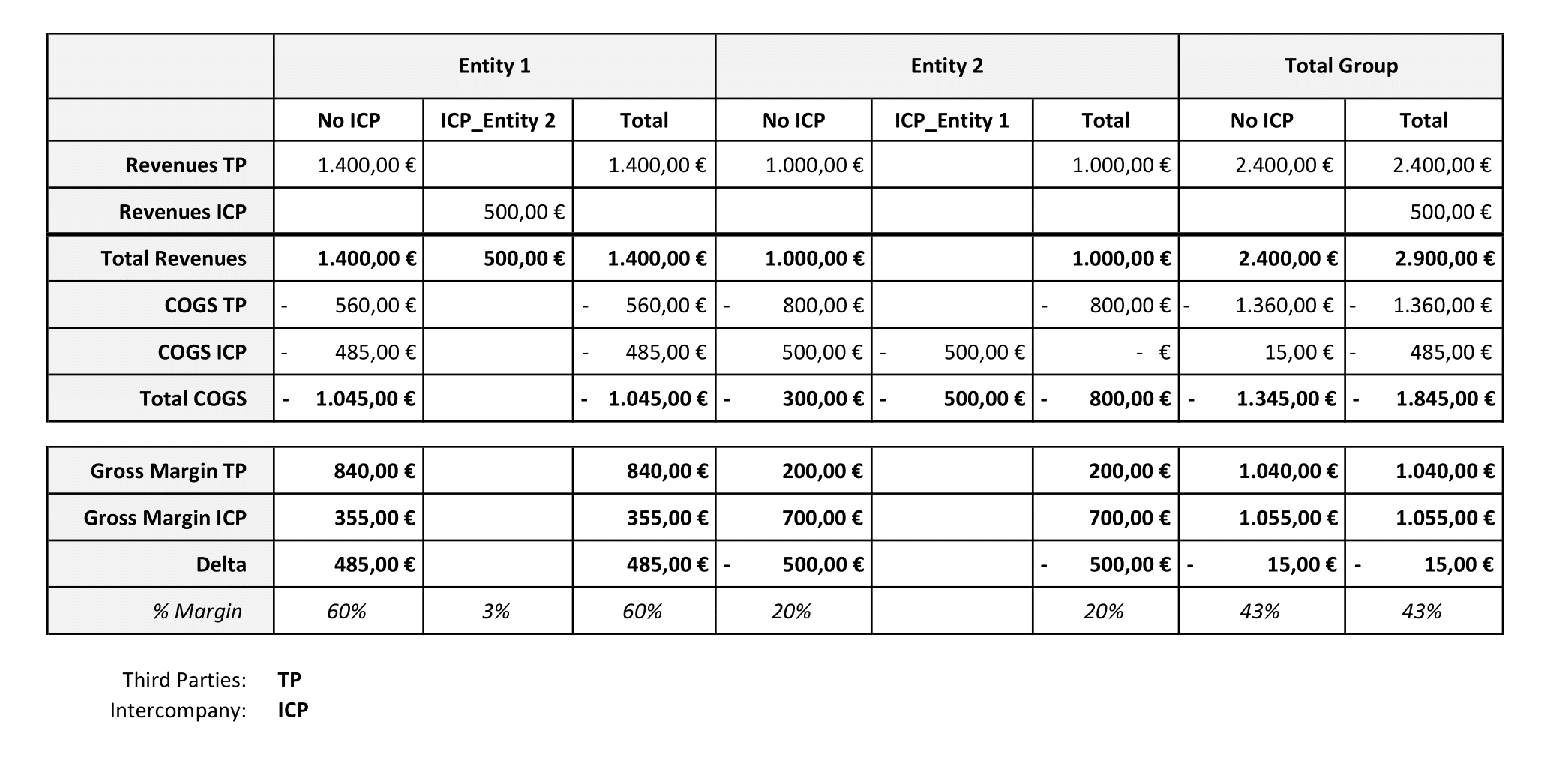
\includegraphics[width=\linewidth]{figures/intercompany.pdf}
	\caption{Intercompany Transaction Logic}
	\label{fig:icp}
\end{figure}

Figure \ref{fig:icp} represents the intercompany transaction logic requested by the Holding Group.
%
The table represents the value of Revenues, Cost of Good Sold (COGS) and Gross Margin, for two entities (Entity 1 and Entity 2), highlighting the presence of the intercompany.
%
In this example, Entity 1 registered a sale transaction of € 500.00 with Entity 2, which registered a COGS for the same amount. 
%
At the same time, Entity 1 registered percentage margin of 3\%, meaning that the COGS for that transaction amounts to € 485.00 (97\% of the revenue).
%
The remaining revenue margin is reflected in the financial view of the Holding Group by checking the difference between the Gross Margin towards third parties and those towards intercompany transactions.
%
This statutory view serves as the starting block on which the consolidated process is built, which represents the overall financial position of the Group as a whole.
%
It provides a comprehensive view that combines the financial information of all the entities and is built by distinguishing two distinct perspectives: the Entity View and the Brand View.

The Entity View focuses on the values at the Entity level, inclusive of intercompany transactions.
%
In this perspective, each individual Entity is treated as a separate reporting unit and the financial information of each Entity, including its assets, liabilities, revenues, and expenses, is consolidated without any eliminations of intercompany transactions. 
%
This approach provides a detailed understanding of each Entity's financial standing and performance, allowing stakeholders to assess the individual contribution of each Entity to the Group as a whole.
%
On the other hand, the Brand View takes into consideration the values at the brand level, with the elimination of intercompany transactions among entities of the same brand group. 
%
Under this perspective, entities within are grouped based on their shared brand and intercompany transactions between entities belonging to the same brand group are eliminated to avoid double-counting and provide a more accurate representation of the brand's financial position and performance. 
%
This approach allows stakeholders to evaluate the financial results specifically related to a particular brand within the Holding Group, enabling strategic decision-making and brand-level performance analysis.

Both the Entity View and Brand View of the consolidated financial statement offer unique insights and serve different purposes. 
%
The Entity View provides a granular understanding of each Entity's financial performance, while the Brand View enables a focused assessment of the performance and financial health of specific brands within the Holding  Group. 
%
The choice between these perspectives depends on the specific needs of stakeholders and the level of detail required for decision-making and analysis.
%
It is worth noting that the Entity View and Brand View are not mutually exclusive, and both perspectives can be presented within a consolidated financial statement. 
%
In this case, the consolidated financial statement includes separate sections that highlight the Entity-level financial information as well as the brand-level financial information after the elimination of intercompany transactions. 
%
This dual perspective provides a comprehensive picture of the Holding Group's financial performance, encompassing both the individual entities and the brands.

Concerning the implementation process of this intercompany solution, to overcome the issue of the restricted access on data belonging to different entities, the system is designed to allow data to be inputted by only one Entity, specifically the one responsible for registering the cost of goods sold (COGS).
%
In this system, the revenues of other entities can be automatically calculated based on a predefined business rule that extract the relevant Entity based on the intersection of dimensions in which the COGS is registered.
%
By designating one Entity as the sole provider of COGS data, the system reduces redundancy and potential errors that may arise from multiple entities independently recording the same transaction. 
%
This Entity becomes the source of reference for determining the cost of goods sold across the Holding Group.
%
At the same time, the entities which register the revenue have the possibility to input the margin which will adjust the value of the cogs related to the specific intercompany transaction.
%
When the COGS data is registered by the designated Entity, the intercompany management system identifies the appropriate dimensions associated with the transaction and the business rules will determine the entities that are impacted by the transaction and calculate the corresponding revenues for each Entity.
%
This automated approach eliminates the need for manual data input and revenue calculations across multiple entities, thus reducing the potential for errors and ensuring consistency in the intercompany reconciliation process. 
%
Furthermore, it provides real-time visibility into intercompany transactions and facilitates efficient and accurate financial reporting and analysis.

\section{Best practices for implementation}

Throughout my experience in the technology - EPM team, I gained valuable insights into best practices for Oracle Cloud EPM implementation and stakeholders management.
%
Here, I reflect on these key takeaways, which encompass data accuracy, stakeholder engagement, clear communication, and continuous improvement.

\paragraph{Data Accuracy:}
One of the fundamental aspects of successful implementation and, in particular, for the implementation of the cost allocation and intercompany management systems, is ensuring data accuracy. 
%
When manipulating data through business rules in an Oracle Cloud EPM implementation, it is essential to prioritize data accuracy and avoid permanently modifying meaningful data. 
%
Before deploying business rules to production, it is important to create test scenarios that cover various data scenarios and performing extensive testing to ensure the rules produce the expected outcomes. 
%
By validating business rules against known data sets, it is possible to identify any discrepancies or unintended consequences and make necessary adjustments to maintain data accuracy.

\paragraph{Stakeholder Engagement:}
Engaging stakeholders at various levels is vital for the success of the implementations. 
%
As I worked on the project, I realized the significance of involving key stakeholders from different departments in the requirements gathering, design, and testing phases. 
%
By actively involving stakeholders, we could gain a deeper understanding of their specific needs and challenges, enabling us to tailor the EPM solution to meet the requirements of the Group effectively.

\paragraph{Clear Communication:}
Clear and effective communication played a key role in the success of the implementations. 
%
This involved breaking down complex concepts into easily understandable terms, providing regular updates on the implementation progress, and addressing any concerns or questions of the client promptly. 
%
By fostering transparent and open communication channels, we could ensure alignment among stakeholders and maintain their support throughout the implementation journey.

\paragraph{Continuous Improvement:}
The implementation of cost allocation and intercompany management is an iterative process that requires continuous improvement. 
%
As we encountered challenges and learned from the practical implementation experience, it became evident that ongoing optimization and refinement were necessary. 
%
This can be done by reviewing the implemented processes and monitoring their performance to identify areas for improvement. \\

During the implementation of the EPM solution in Oracle Cloud EPM, I gained several valuable insights that have contributed to the successful deployment of the system.
%
This experience provided a deeper understanding of the benefits and challenges associated with leveraging business rules within the EPM solution for complex organizational structures like Holding Groups.
%
One of the key insights gained was the ability of business rules to streamline and automate complex financial calculations: business rules offered a powerful tool to define and execute calculations, consolidations, allocations, and eliminations across the different entities. 
%
Another important insight was the importance of collaboration and coordination among stakeholders during the design and implementation of the process. 
%
Given the diversified nature of the Holding Group, it was crucial to engage effective communication with the client in order to collect requirements effectively and receive feedback continuously.
%
An important challenge that emerged during the implementation was the need for focused testing and validation of complex business rules as, due to the intricacies of the Group's financial structure, it was crucial to conduct comprehensive testing to ensure the accuracy and integrity of the calculations. 
%
Developing a robust testing framework, including test scenarios, data sets, and validation procedures, was critical to mitigating potential errors and identifying any anomalies before deploying to production.
%
In conclusion, the implementation of this EPM solution provided valuable insights into the benefits and challenges associated with leveraging business rules for complex financial structures. 
%
Through automation, collaboration, flexibility, and comprehensive testing, the implementation successfully integrated the EPM solution into the organization's financial management practices, driving better decision-making and optimizing performance across the Holding Group.

%----------------------------------------------------------------------------------------
\chapter{\conclusionsname}
\label{chap:conclusions}
%----------------------------------------------------------------------------------------

\section{Summary of the project}

\section{Discussion and concluding thoughts}


%----------------------------------------------------------------------------------------
% BIBLIOGRAPHY
%----------------------------------------------------------------------------------------

\nocite{*} % uncomment this to show all the reference in the .bib file
\bibliographystyle{plain}
\bibliography{bibliography}


\end{document}